%\documentclass{article}
%\usepackage[utf8]{inputenc}
%
%\title{covid19-eda}
%\author{ckatsak }
%\date{January 2021}
%
%\usepackage{natbib}
%\usepackage{graphicx}
%
%\begin{document}
%
%\maketitle
%
%\section{Introduction}
%There is a theory which states that if ever anyone discovers exactly what the Universe is for and why it is here, it will instantly disappear and be replaced by something even more bizarre and inexplicable.
%There is another theory which states that this has already happened.

%\begin{figure}[h!]
%\centering
%
\includegraphics[scale=1.7]{images/pyrforos.jpg}
%\caption{The Universe}
%\label{fig:universe}
%\end{figure}
%
%\section{Conclusion}
%``I always thought something was fundamentally wrong with the universe'' \citep{adams1995hitchhiker}
%
%\bibliographystyle{plain}
%\bibliography{references}
%\end{document}




%%======================================================================================
%%======================================================================================





\documentclass[12pt]{article}
\usepackage[utf8]{inputenc}
\usepackage[greek,english]{babel}
\usepackage[margin=2cm]{geometry}
\usepackage{alphabeta}
\usepackage{booktabs}
\usepackage{listings}
\usepackage{amsmath}
\usepackage{amssymb}
\usepackage[unicode]{hyperref}
\usepackage{bookmark}
\usepackage{fancyhdr}
\usepackage[nottoc]{tocbibind}
\usepackage{tabto}
\usepackage{stackengine}

\usepackage[makeroom]{cancel}

\usepackage{hhline}
\usepackage[export]{adjustbox}
\usepackage[font=footnotesize, justification=centering]{caption}
\usepackage{subcaption}
\usepackage{chngcntr}

\usepackage{makecell}
\usepackage{enumitem}

\usepackage{afterpage}
\usepackage{lastpage} %% for `\pageref{LastPage}` reference

\newcommand\blankpage{%
	\null%
	\thispagestyle{empty}%
	\addtocounter{page}{-1}%
	\newpage%
}

\hypersetup{
    colorlinks,
	citecolor = black,
	filecolor = black,
	linkcolor = black,
	urlcolor = black
}

\usepackage{indentfirst}

\usepackage{titlesec}
\usepackage{titling,multicol}
\usepackage[most]{tcolorbox}
\usepackage{float}
\usepackage[useregional]{datetime2}
\usepackage{datetime}
%\usepackage{pgfplots}
\usepackage{relsize}

\usepackage[labelfont=bf]{caption}
\usepackage[font=footnotesize, justification=centering]{caption}
\usepackage{array}

\fancypagestyle{styletoc}{% <===========================================
    \lhead{Table of Contents}
    \rhead{}
    \cfoot{Page \thepage}
    %\renewcommand{\headrulewidth}{0pt}
}
\fancypagestyle{styleimage}{% <===========================================
    %\lhead{List of Figures}  %% better show ToC when they're on the same page
    \rhead{}
    \cfoot{Page \thepage}
    %\renewcommand{\headrulewidth}{0pt}
}
\fancypagestyle{styletotal}{% <===========================================
    \lhead{\nouppercase{\leftmark}}
    \rhead{Section \thesection}
    %\cfoot{Page \thepage}
    \cfoot{Page \thepage\ of \pageref{LastPage}}
    %\renewcommand{\headrulewidth}{0pt}
}

\hypersetup{
	colorlinks,
	citecolor = black,
	filecolor = black,
	linkcolor = black,
	urlcolor = black
}
%\usepackage[bottom]{footmisc}
\pagestyle{fancy}
\fancyhf{}
\lhead{\nouppercase{\leftmark}}
\rhead{Section \thesection}
\cfoot{Page \thepage}
%\renewcommand{\footrulewidth}{0.5pt}% default is 0pt
\renewcommand{\footrulewidth}{0.1pt}% default is 0pt
\makeatletter
\DeclareMathOperator*{\argmax}{argmax} % thin space, limits underneath in displays
\addto{\captionsenglish}{\renewcommand{\bibname}{Bibliography}}

\addto\captionsenglish{% Replace "english" with the language you use
	\renewcommand{\contentsname}%
	{Table of Contents}%
}

\addto\captionsenglish{% Replace "english" with the language you use
	\renewcommand{\listfigurename}%
	{List of Figures}%
}

\addto\captionsenglish{\renewcommand{\chaptername}{Chapter}}

\addto\captionsenglish{\renewcommand{\figurename}{\textbf{Figure}}}

\addto\captionsenglish{\renewcommand{\tablename}{Table}}

\hypersetup{
	colorlinks,
	citecolor = black,
	filecolor = black,
	linkcolor = black,
	urlcolor = blue
}

%\usepackage{xcolor}
%% Use minted for more decent listing styling.
%% Also see https://tex.stackexchange.com/q/24945 for line refs in minted listings.
\usepackage{minted}
\usemintedstyle{emacs}
%\usemintedstyle{manni}
%\usemintedstyle{friendly}
%\usemintedstyle{perldoc}

\begin{document}

	\begin{titlepage}
		\newcommand{\HRule}{\rule{\linewidth}{0.1mm}}
		\center
		\textsc{\Large National Technical University of Athens}\\[0.5cm]
		%\textsc{\large ΔΠΜΣ Επιστήμη Δεδομένων και Μηχανική Μάθηση}\\[1.0cm]
		\vspace{1cm}
		
\includegraphics[scale=0.2]{images/pyrforos.jpg}\\[1cm]
		\textsc{\large Programming Tools and Technologies for Data Science}\\[0.5cm]

		%\HRule \\[0.2cm]
		\HRule \\[0.2cm]

		\textsc{\Large Exploratory Data Analysis \\ \large of CSSE's COVID-19 Dataset}\\

		%\HRule \\[1cm]
		\HRule \\[2cm]

		%\Large \underline{ΟΜΑΔΑ 7}\\
		\vspace{0.5cm}

	 	\Large
		Christos Katsakioris\\
		ckatsak@cslab.ece.ntua.gr\\
		03002964\\
		\vspace{0.25cm}
		\large
		PhD Candidate\\
		Computing Systems Laboratory\\
		School of Electrical and Computer Engineering\\

		\vspace{3.5cm}
		\center Athens, Greece
		\center {\selectlanguage{english}\today}\\[2cm]
	\end{titlepage}

    \pagenumbering{roman}
    \pagestyle{styletoc}{
        \tableofcontents
        %\newpage  %% (Un)comment to toggle `List of Figures` being on the same page as ToC
    }
    \pagestyle{styleimage}{
	    \listoffigures
	    \newpage
	}

	\pagestyle{styletotal}
    \pagenumbering{arabic}

	\section{Introduction}

This work is a basic Exploratory Data Analysis of the COVID-19 Data provided by the Center for Systems Science and Engineering (CSSE) at Johns Hopkins University\cite{ghcsse}.

For the development, I leveraged the power of the R language on a GNU/Linux \texttt{x86\_64} platform, as provided through the official \texttt{r-base} Docker images\cite{dhrbase} of the project (which are based on the Debian \texttt{testing} release), as well as the \texttt{Vim}\cite{vim} text editor.

The development has relied upon the modern principles of structured programming and taken place in a modular, function-based fashion, rather than employing a non-modular, top-down scripting process.
As a disclaimer, and with respect to this assignment's requirements to include the code within this document \textit{and} to not exceed the limit of $15$ pages, this practice might sometimes be convenient, but it might as well sometimes be not.
%TODO: repo
In any case, the source code has been made publicly available in its whole for further inspection; it is hosted on GitHub and can be accessed at \url{https://github.com/ckatsak/covid-eda-r}.
%TODO: repo
	\section{Initial Processing}


\subsection{Entry Point}

Omitting the shebang declaration, the introductory and documentation comments and the definition of global constants, we begin by importing the libraries upon which there is dependence:

\begin{minted}[linenos = true]{R}
library(data.table) # for all sorts of processing
library(lubridate)  # for `mdy()`
library(ggplot2)    # for plotting
\end{minted}

The number of external dependencies has been deliberately kept to a minimum, to ease our procedure's reproducibility in the context of the course.

At the bottom of the source code file, we define the entry point of our program.
This is merely an output width configuration for the case of interactive execution, or a \texttt{main()} function otherwise.

\begin{minted}[linenos = true]{R}
main <- function() {
  eda(processing()$dt)
}

if (interactive()) {
  options("width" = 120)
} else {
  main()
}
\end{minted}


\subsection{Processing Steps}

Let us start by focusing on the processing of the given dataset following the given instruction steps of the assignment.
All of the processing has been included in a single R function, \texttt{processing()}.

\begin{minted}[linenos=true, escapeinside=@@]{R}
processing <- function() {
  # (Down)load the latest data into a new data.table, excluding some columns
  exclusions <- c("Province/State", "Lat", "Long")
  confirmed  <- fread(CONFIRMED_URL, header = TRUE, drop = exclusions)
  deaths     <- fread(DEATHS_URL,    header = TRUE, drop = exclusions)

  # Appropriately rename the variable related to the country
  setnames(confirmed, "Country/Region", "Country")
  setnames(deaths,    "Country/Region", "Country")

  # Reshape each data.table from wide to long format
  confirmed <- melt(confirmed, id.vars = c("Country"), variable.name = "date",
                    value.name = "confirmed", variable.factor = FALSE)
  deaths    <- melt(deaths,    id.vars = c("Country"), variable.name = "date",
                    value.name = "deaths",    variable.factor = FALSE)

  # Convert each date variable from character to a date object using `mdy()`
  confirmed <- confirmed[, date := mdy(date)]
  deaths    <- deaths[   , date := mdy(date)]

  # Group them by (Country, date) summing deaths
  confirmed <-confirmed[, .(confirmed = sum(confirmed)), by = .(Country, date)]
  deaths    <-deaths[   , .(deaths    = sum(deaths)),    by = .(Country, date)]

  # Merge the two datasets into one
  dt <- merge(confirmed, deaths)

  # Calculate the total number of confirmed cases as well as the total number
  # of deaths, worldwide
  #
  # NOTE: Since the recorded data are cumulative, σ(most_recent) -> aggregate
  confirmed <- sum(dt[date == max(date)][, confirmed])
  deaths    <- sum(dt[date == max(date)][, deaths])

  # Sort by country and date
  dt <- dt[order(Country, date)]

  # Calculate daily increases
  dt[, ":="(
       confirmed.ind = confirmed - shift(confirmed, 1, type = "lag", fill = 0),
       deaths.inc    = deaths    - shift(deaths,    1, type = "lag", fill = 0)
     ),
     by = .(Country)
  ]

  # Return the results as a list
  ret <- list(confirmed, deaths, dt)
  names(ret) <- c("confirmed", "deaths", "dt")
  ret
}
\end{minted}

Rather than repeating the explanation of the implementation of each step, we have annotated the source code in the above listing with comments that indicate the effects of each of the included statements.
We explicitly note, however, that step 1 has been merged with the code for the initial retrieval of the data in the beginning of the function, step 3 has preceded step 2 in our implementation, and step 10 leverages \texttt{data.table}'s \texttt{shift()} function specifying the \texttt{type} parameter equal to \texttt{"lag"} (rather than employing the \texttt{lag()} function of the \texttt{stats} package).

	\section{Aggregate Stats}

The EDA is bootstrapped through the following function, which is called by function \texttt{main()}:

\begin{minted}[linenos = true]{R}
eda <- function(dt) {
  plot_summary(calc_summary(dt))
  plot_seasons(determine_hemispheres(dt))
}
\end{minted}

This section focuses on the first part of the conducted EDA, which addresses aggregate statistics deduced from the dataset.
These are calculated in \texttt{calc\_summary()} and plotted (after being further processed) in \texttt{plot\_summary()}.

\begin{minted}[linenos = true, escapeinside=@@]{R}
calc_summary <- function(dt) {
  countries <- unique(dt$Country)
  aggr_dt <- function(group) {                                    @\label{aggr_dt_A}@
    dt[Country %in% group,
       .(
         total.deaths         = sum(deaths.inc),
         total.confirmed      = sum(confirmed.ind),
         total.ratio          = sum(deaths.inc) / sum(confirmed.ind),
         mean.daily.confirmed = mean(confirmed.ind),
         mean.daily.deaths    = mean(deaths.inc)
        ),
       by = .(Country)]
  }                                                               @\label{aggr_dt_Z}@
  all_agdt <- aggr_dt(countries)
  mean_dt <- function(name, group) {                              @\label{mean_dt_A}@
    all_agdt[Country %in% group,
             .(
               Country              = name,
               total.deaths         = sum(total.deaths),
               total.confirmed      = sum(total.confirmed),
               total.ratio          = mean(total.ratio),
               mean.daily.confirmed = mean(mean.daily.confirmed),
               mean.daily.deaths    = mean(mean.daily.deaths)
              )]
  }                                                               @\label{mean_dt_Z}@
  world <- mean_dt("WORLD", countries)                            @\label{calc_sum_1}@
  eu    <- mean_dt("EUROPEAN UNION", EU)
  nord  <- mean_dt("NORDIC COUNTRIES", NORDIC)
  brics <- mean_dt("BRICS", BRICS)
  balk  <- mean_dt("BALKAN COUNTRIES", BALKANS)
  gulf  <- mean_dt("GULF COUNTRIES", GULF)                        @\label{calc_sum_2}@

  rbind(all_agdt, world, eu, nord, brics, balk, gulf)             @\label{calc_sum_ret}@
}
\end{minted}

Function \texttt{calc\_sum()}, using the auxiliary function \texttt{aggr\_dt} (lines \ref{aggr_dt_A}-\ref{aggr_dt_Z}) and the closure \texttt{mean\_dt} over the local variable \texttt{all\_agdt} (lines \ref{mean_dt_A}-\ref{mean_dt_Z}), calculates the aggregate statistics for some predefined geographic and economic groups of countries that would be interesting to compare (lines \ref{calc_sum_1}-\ref{calc_sum_2}), and returns them through the enrichment of the initially given \texttt{data.table} (line \ref{calc_sum_ret}).

The resulting \texttt{data.table} is piped into the \texttt{plot\_summary} function, which further transforms it to facilitate and conduct the creation of the plots.

In the following listing, lines \ref{econ_A}-\ref{econ_Z} create a temporary factor variable and two stack barplots (Figures \ref{fig:aggr_econ_conf} and \ref{fig:aggr_econ_deaths}) for the total confirmed COVID-19 cases and the total deaths attributed to the virus, respectively, for three major economic groups of countries: the European Union, the BRICS (Brazil, Russia, India, China and South Africa) and the US (which is considered as a whole separate economy here, due to both its vast size and its unique structure).

Subsequently, lines \ref{geo_A}-\ref{geo_Z} repeat a similar procedure, though this time for geographic groups: countries that are mostly or partially ($>= 25\%$ of their area) in the Balkan Peninsula according to \cite{wikibalkans}, the countries that constitute the Arab states of the Persian Gulf according to \cite{wikigulf} and the Nordic countries. 
These are presented in Figures \ref{fig:aggr_geo_conf} and \ref{fig:aggr_geo_deaths}.

\begin{minted}[linenos = true, escapeinside=@@]{R}
plot_summary <- function(dt) {
  # Stack barplots for economic groups                               @\label{econ_A}@
  econ <- dt[Country %in% c(EU, BRICS, "US")
            ][, econ.grp := as.factor(ifelse(Country %in% EU,
                                             "European Union",
                                             ifelse(Country %in% BRICS,
                                                    "BRICS",
                                                    "US")))]
  ggplot(econ) + aes(x = econ.grp, y = total.confirmed, fill = Country) +
    geom_bar(position = "stack", stat = "identity") +
    labs(title = "Confirmed COVID-19 cases per economic group") +
    labs(subtitle = "Dataset from CSSE, Johns Hopkins University") +
    labs(x = "", y = "Confirmed COVID-19 Cases") + theme_bw() +
    geom_text(aes(label = Country), position = position_stack(vjust=.5), size=2)
  ggsave("aggr_econ_conf.png")
  ggplot(econ) + aes(x = econ.grp, y = total.deaths, fill = Country) +
    geom_bar(position = "stack", stat = "identity") +
    labs(title = "COVID-19 deaths per economic group") +
    labs(subtitle = "Dataset from CSSE, Johns Hopkins University") +
    labs(x = "", y = "COVID-19 Deaths") + theme_bw() +
    geom_text(aes(label = Country), position = position_stack(vjust=.5), size=2)
  ggsave("aggr_econ_deaths.png")                                     @\label{econ_Z}@
  
  # Stack barplots for geographic groups                             @\label{geo_A}@
  geogr <- dt[Country %in% c(BALKANS, NORDIC, GULF)
             ][, geo.grp := as.factor(ifelse(Country %in% BALKANS,
                                              "Balkan",
                                              ifelse(Country %in% NORDIC,
                                                     "Nordic",
                                                     "Gulf")))]
  ggplot(geogr) + aes(x = geo.grp, y = total.confirmed, fill = Country) +
    geom_bar(position = "stack", stat = "identity") +
    labs(title = "Confirmed COVID-19 cases per geographic group") +
    labs(subtitle = "Dataset from CSSE, Johns Hopkins University") +
    labs(x = "", y = "Confirmed COVID-19 Cases") + theme_bw() +
    geom_text(aes(label = Country), position = position_stack(vjust=.5), size=2)
  ggsave("aggr_geo_conf.png")
  ggplot(geogr) + aes(x = geo.grp, y = total.deaths, fill = Country) +
    geom_bar(position = "stack", stat = "identity") +
    labs(title = "COVID-19 deaths per geographic group") +
    labs(subtitle = "Dataset from CSSE, Johns Hopkins University") +
    labs(x = "", y = "COVID-19 Deaths") + theme_bw() +
    geom_text(aes(label=Country), position=position_stack(vjust=.5), size=2)
  ggsave("aggr_geo_deaths.png")                                      @\label{geo_Z}@
  
  # Lollipop plots for death-to-confirmed ratios                     @\label{ratio_A}@
  aggrs <- c("WORLD", "EUROPEAN UNION", "NORDIC COUNTRIES", "BRICS",
             "BALKAN COUNTRIES", "GULF COUNTRIES", "US")
  bottom25 <- dt[!Country %in% c("MS Zaandam", "Diamond Princess")
                ][order(-total.ratio)][1:25]
  ratioz <- rbind(dt[Country %in% aggrs], bottom25)[order(-total.ratio)]
  ratioz$Country <- reorder(ratioz$Country, ratioz$total.ratio)
  ggplot(ratioz) + aes(x = Country, y = total.ratio) +
    geom_segment(aes(x = Country, xend = Country, y = 0, yend = total.ratio),
                 color = ifelse(ratioz$Country %in% aggrs, "blue", "dark red"),
                 size  = ifelse(ratioz$Country %in% aggrs, 1.3, 0.7) ) +
    geom_text(aes(label=sprintf("%d out of %d", total.deaths,total.confirmed)),
              vjust = .5, hjust = -.15, color="magenta", size = 1.5) +
    ylim(c(0, .31)) +
    geom_point(color = ifelse(ratioz$Country %in% aggrs, "blue", "dark red"),
               size  = ifelse(ratioz$Country %in% aggrs, 3, 1)) +
    coord_flip() + labs(x = "", y = "Ratio") + theme_bw() +
    labs(title = "Ratio of COVID-19 Deaths to Confirmed COVID-19 Cases") +
    labs(subtitle = "Dataset from CSSE, Johns Hopkins University")
  ggsave("aggr_ratio_lollipop.png")                                  @\label{ratio_Z}@
}
\end{minted}

\begin{figure}[H]
\centering
\begin{minipage}{.5\textwidth}
  \centering
  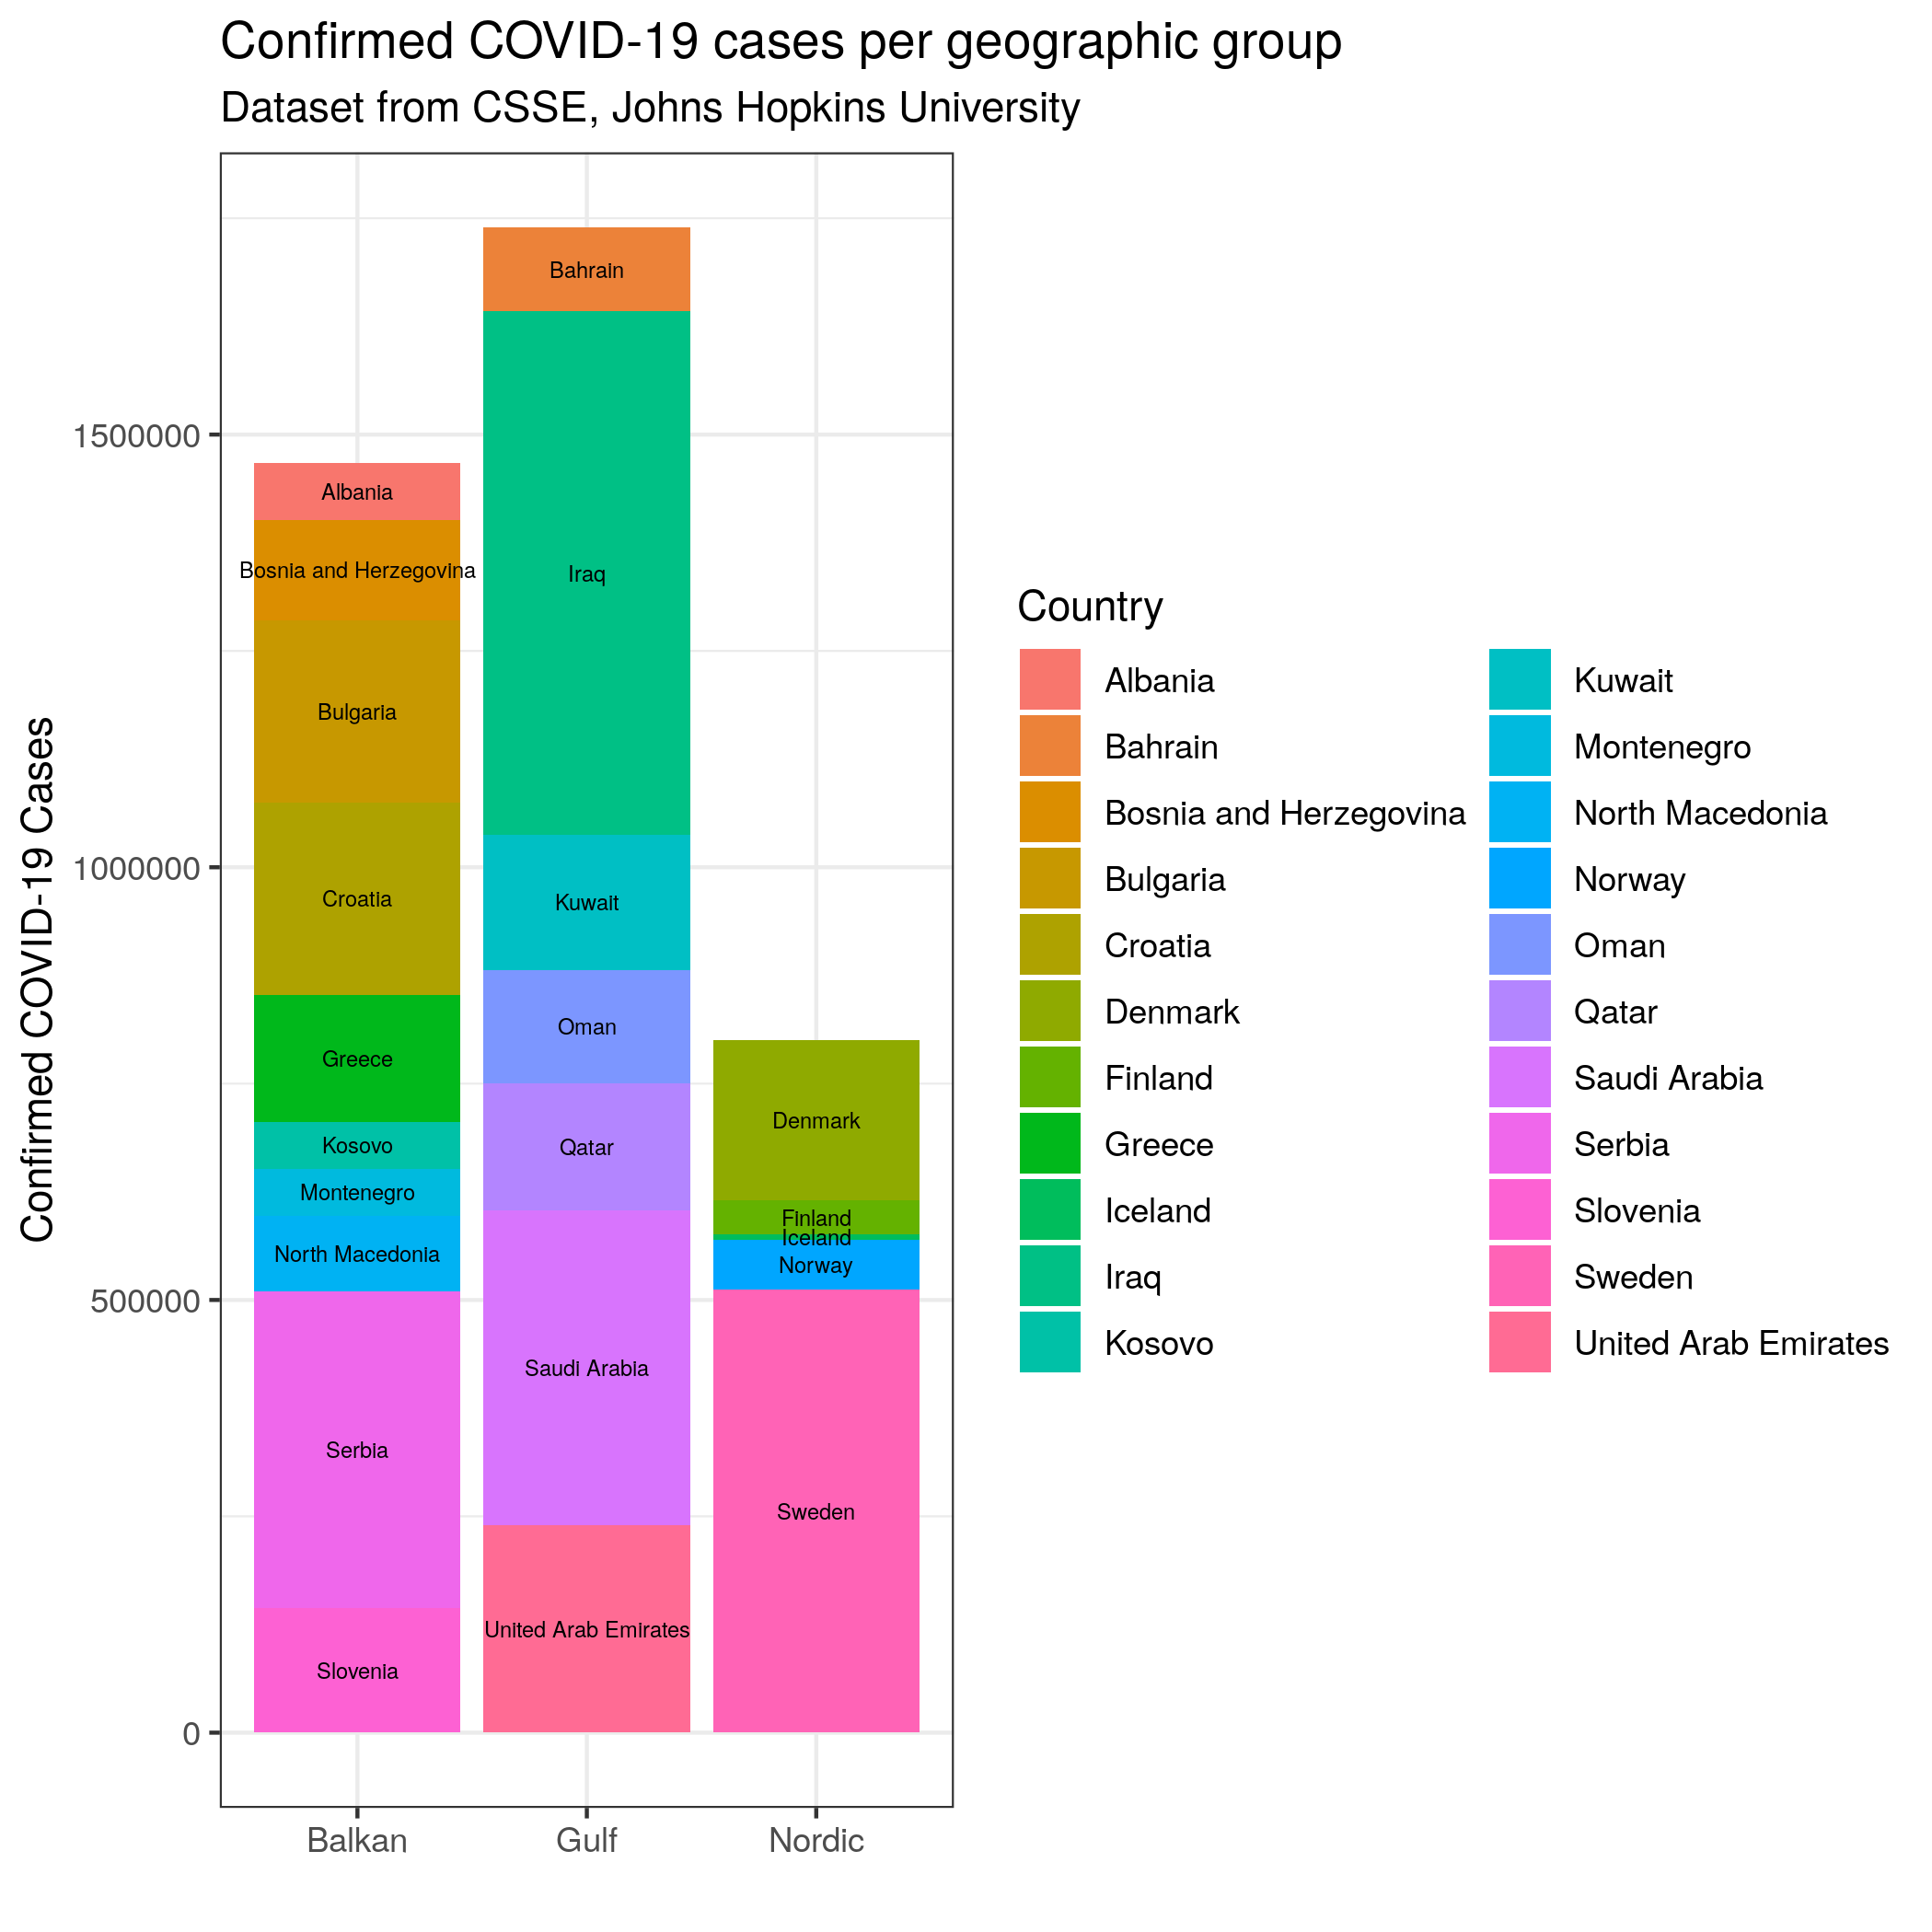
\includegraphics[width=1\linewidth]{images/aggr_geo_conf.png}
  \captionof{figure}{Confirmed COVID-19 cases per geographic group}
  \label{fig:aggr_geo_conf}
\end{minipage}%
\begin{minipage}{.5\textwidth}
  \centering
  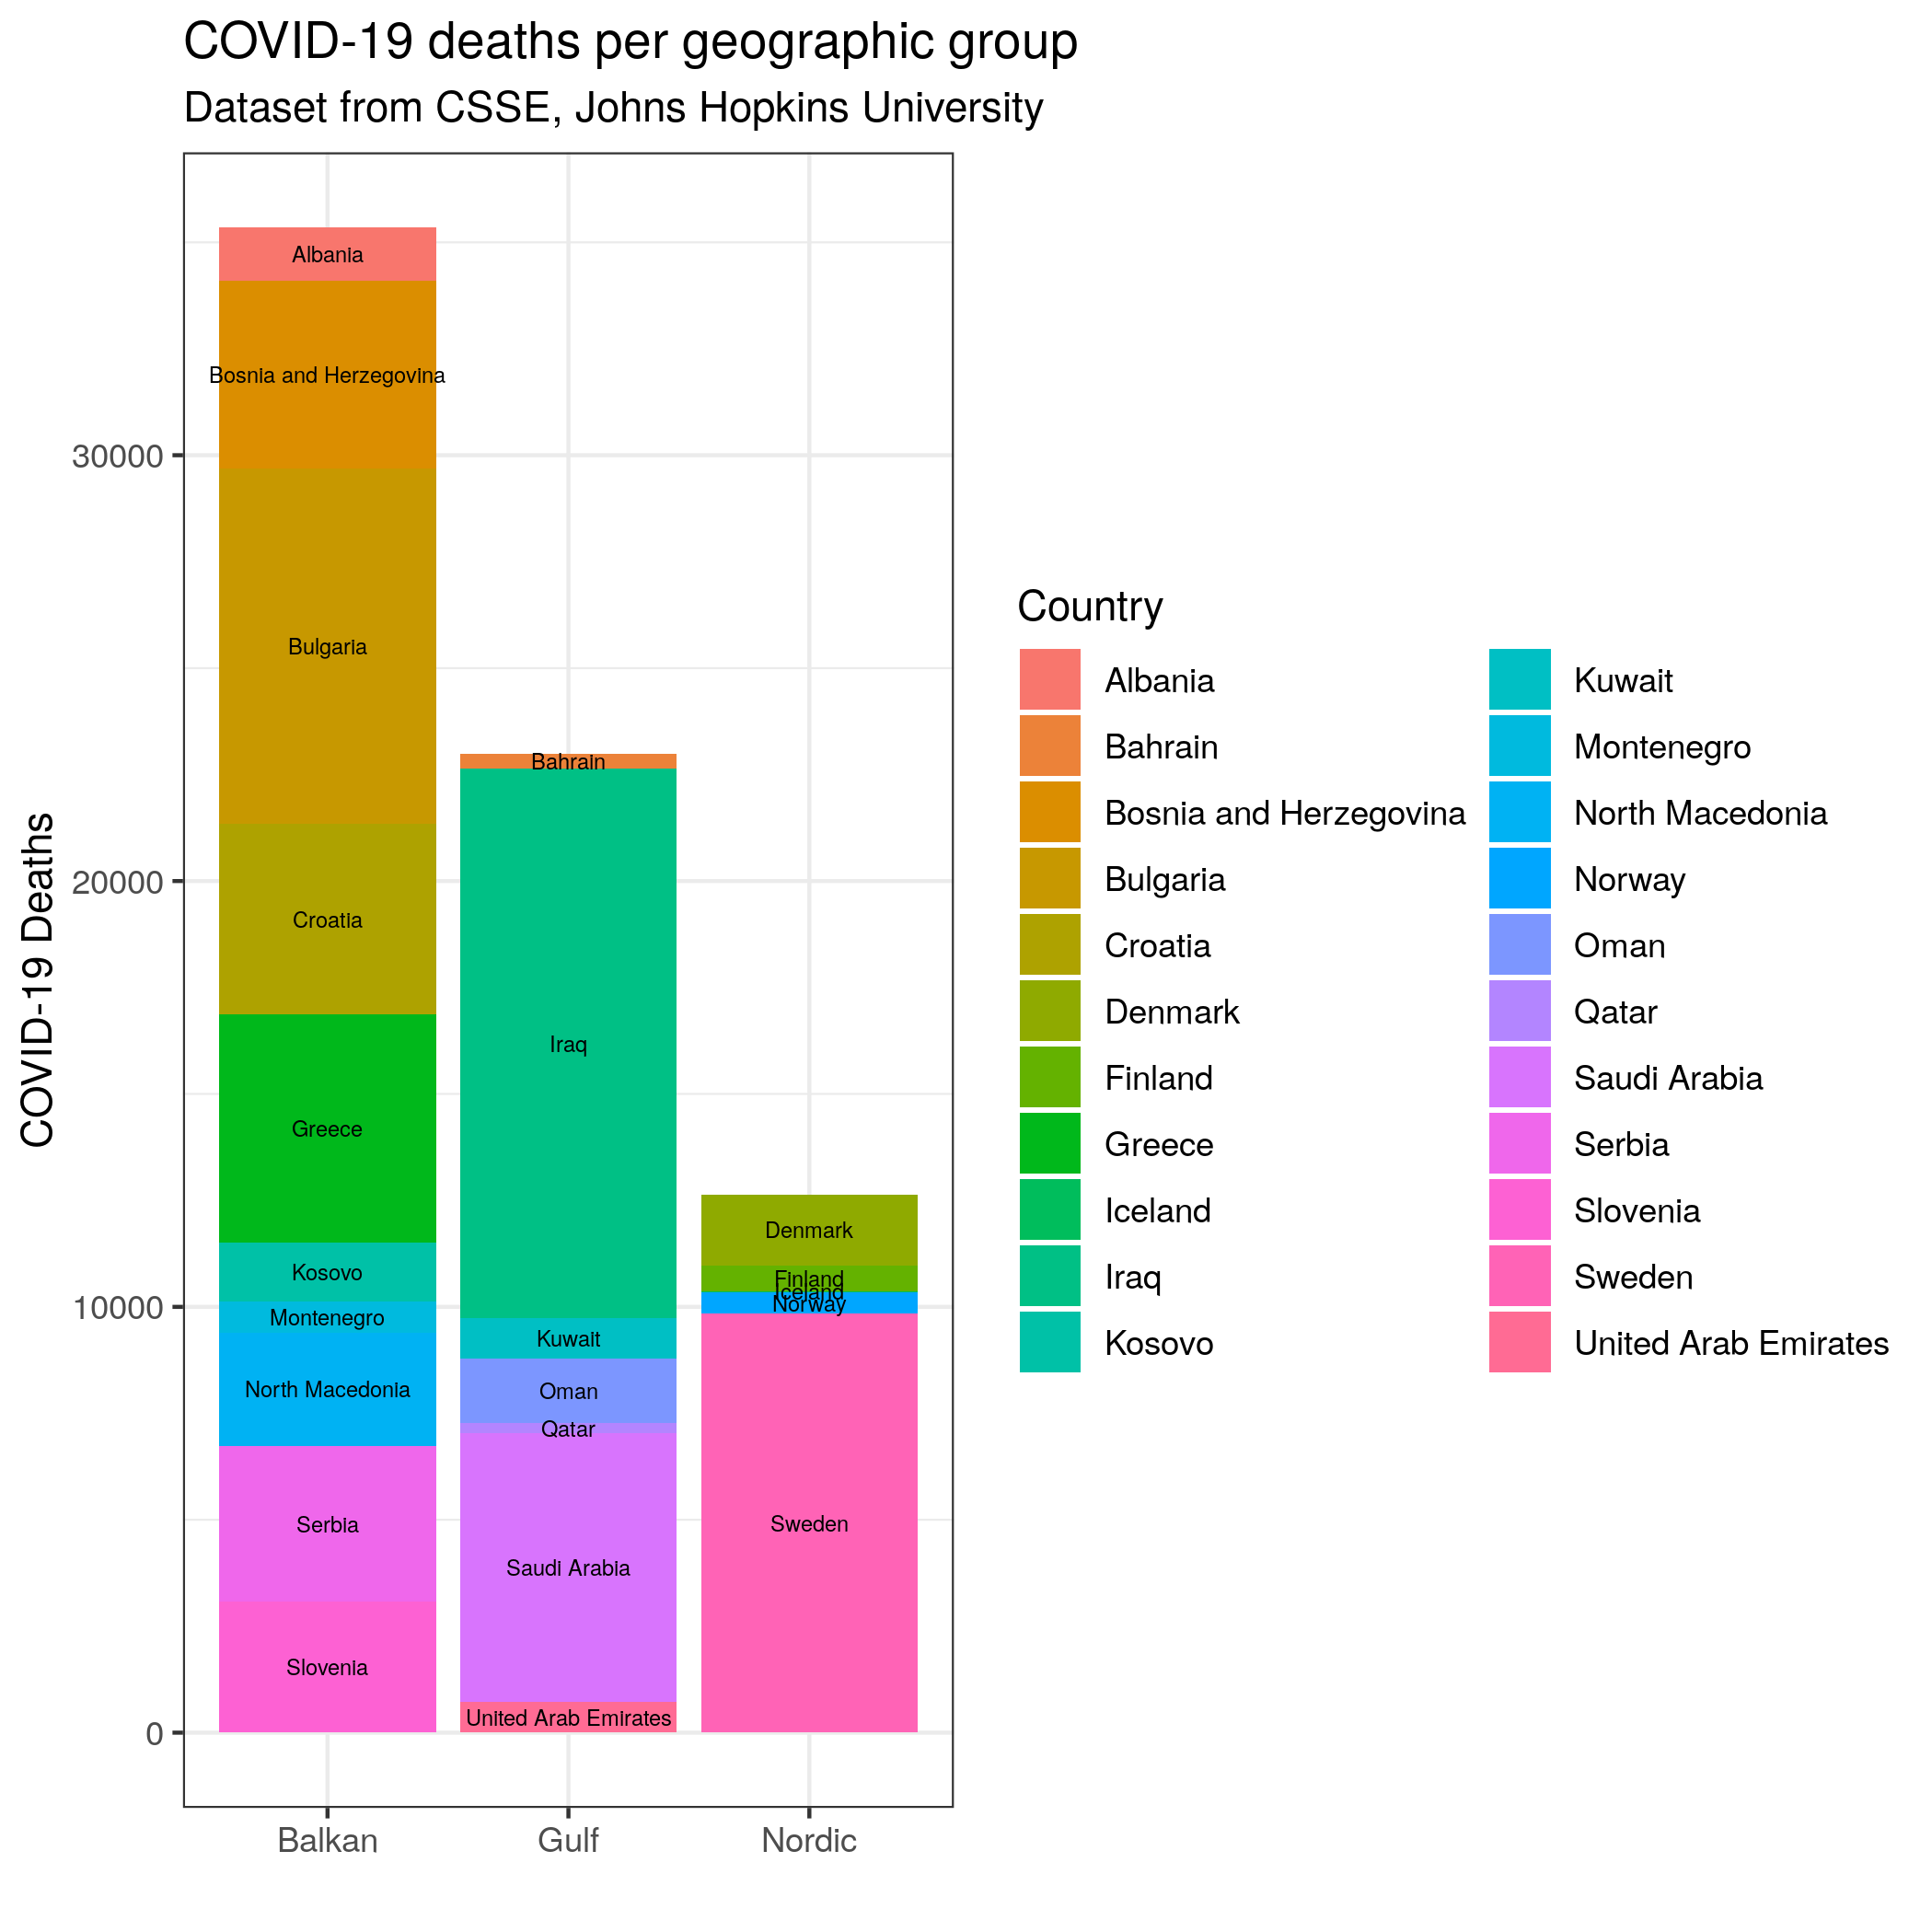
\includegraphics[width=1\linewidth]{images/aggr_geo_deaths.png}
  \captionof{figure}{COVID-19 deaths per geographic group}
  \label{fig:aggr_geo_deaths}
\end{minipage}
\end{figure}

\begin{figure}[H]
\centering
\begin{minipage}{.5\textwidth}
  \centering
  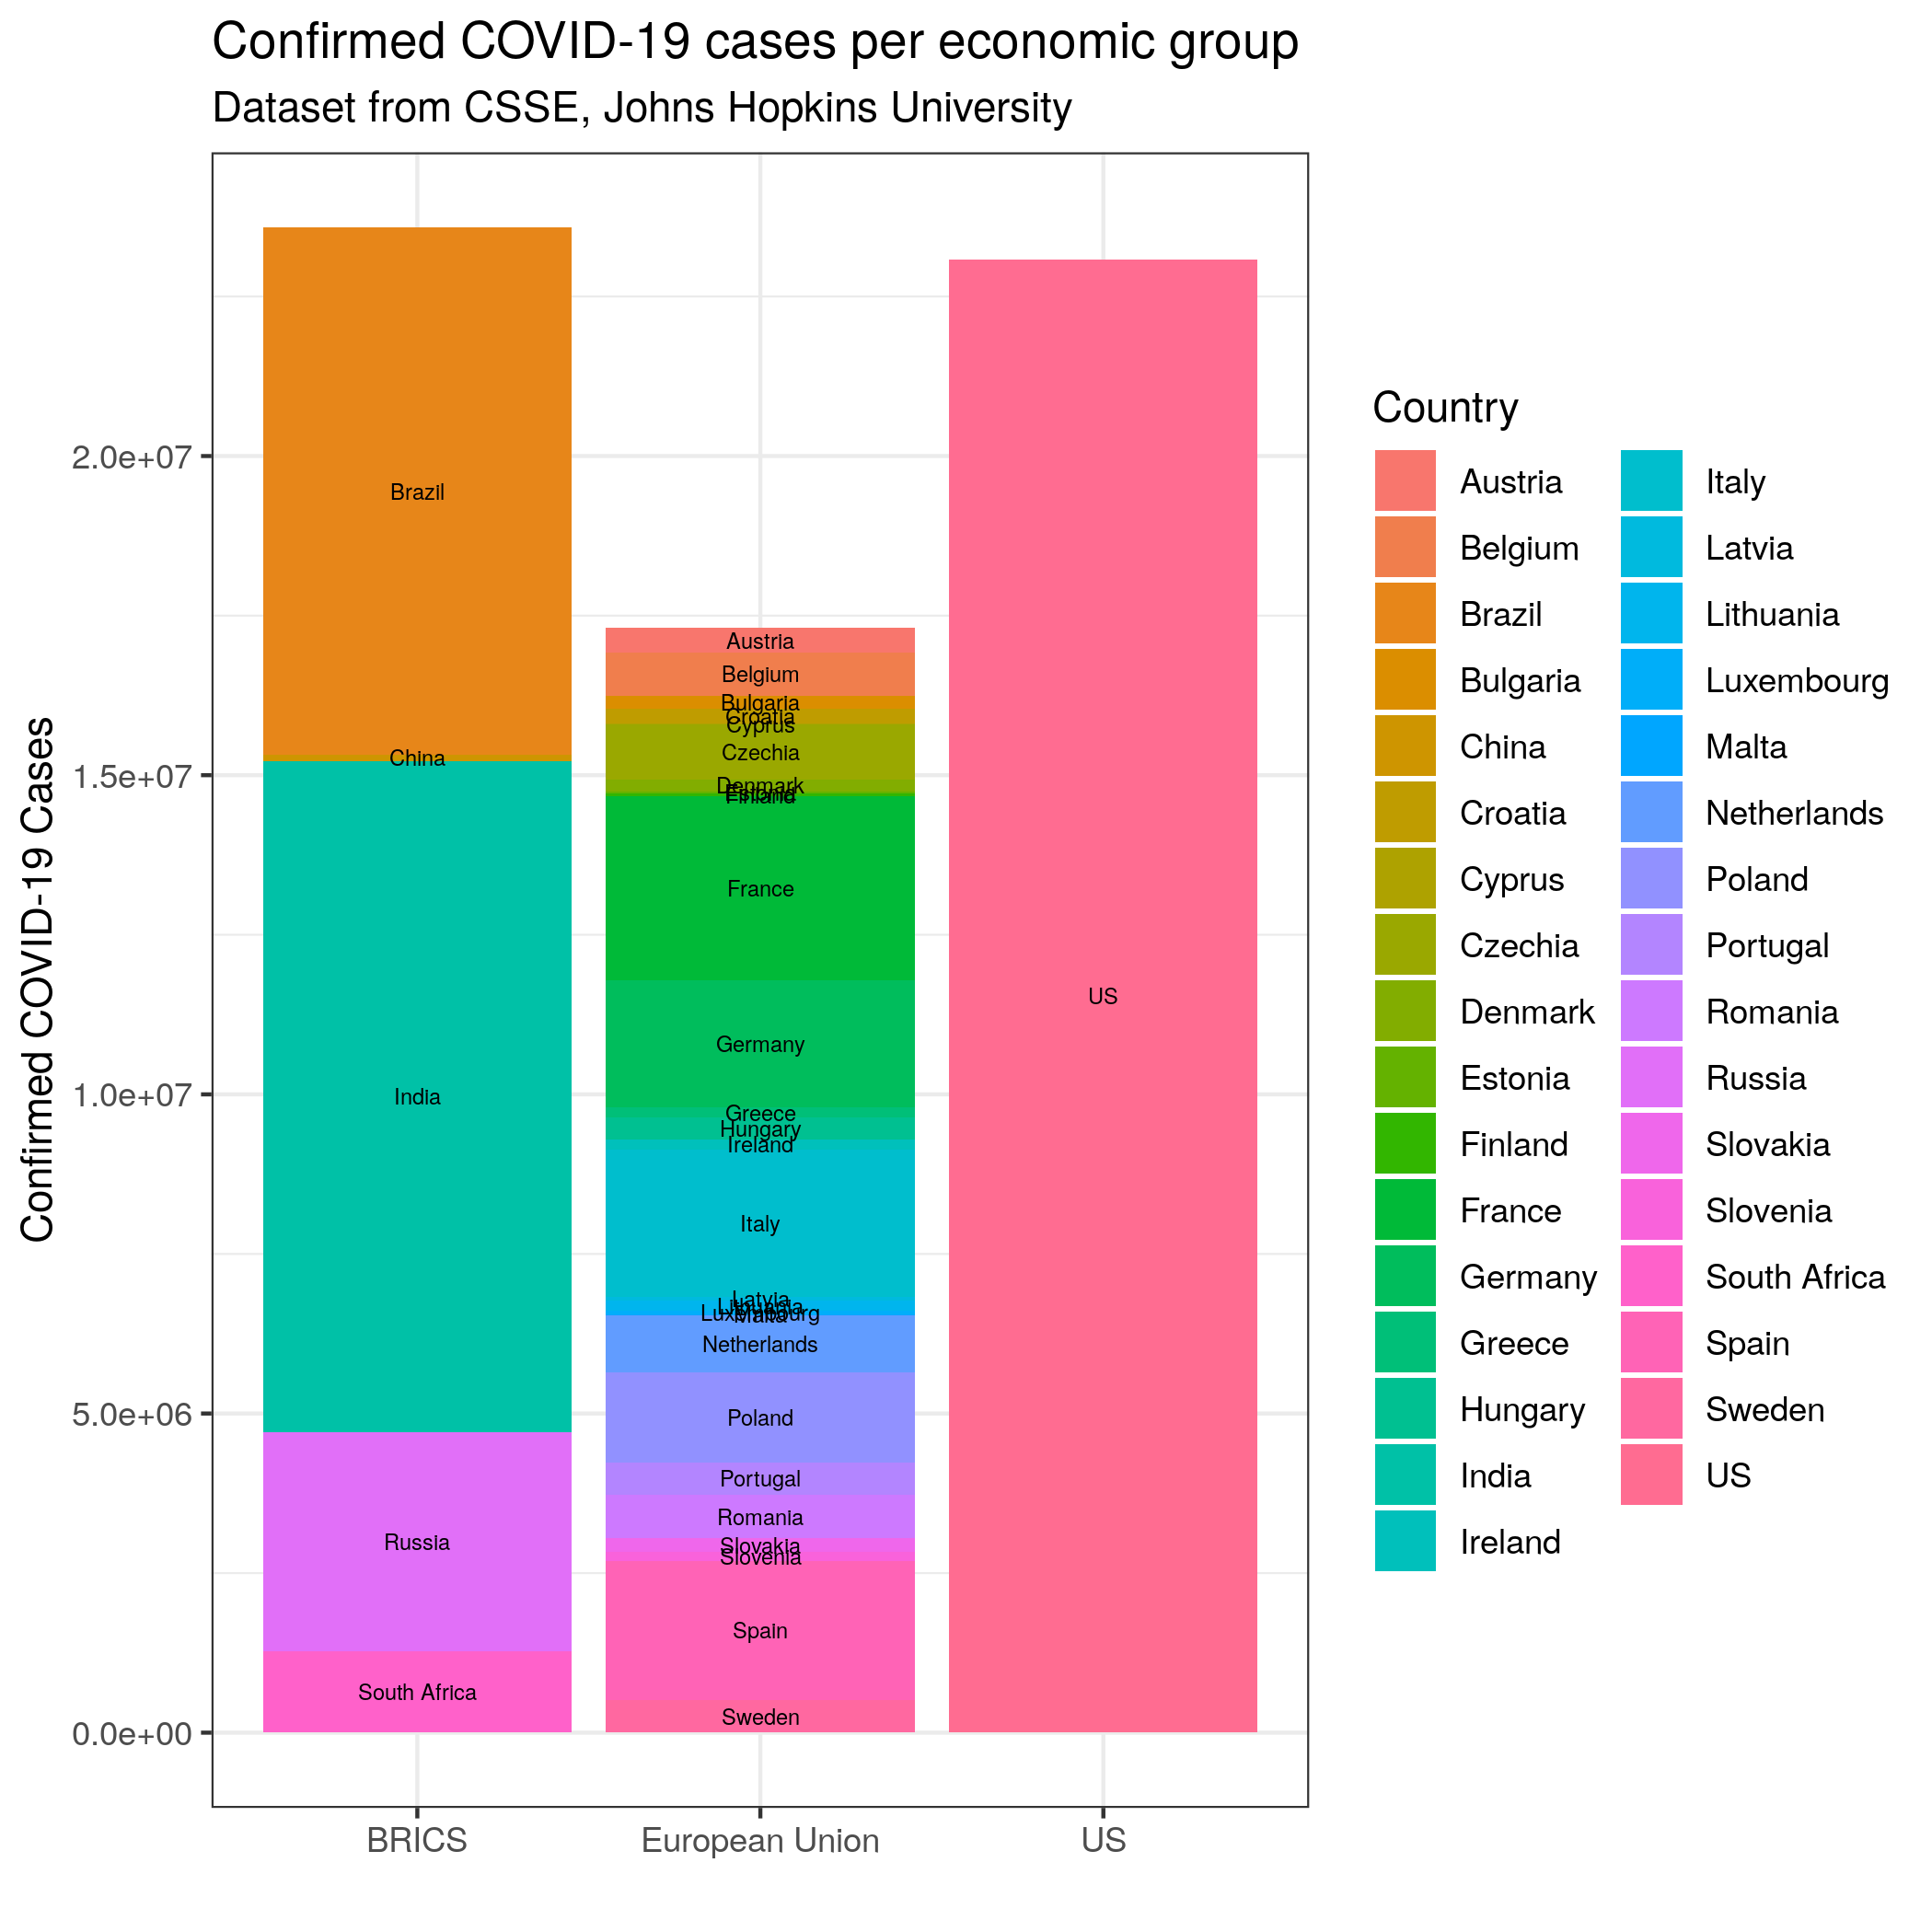
\includegraphics[width=1\linewidth]{images/aggr_econ_conf.png}
  \captionof{figure}{Confirmed COVID-19 cases per economic group}
  \label{fig:aggr_econ_conf}
\end{minipage}%
\begin{minipage}{.5\textwidth}
  \centering
  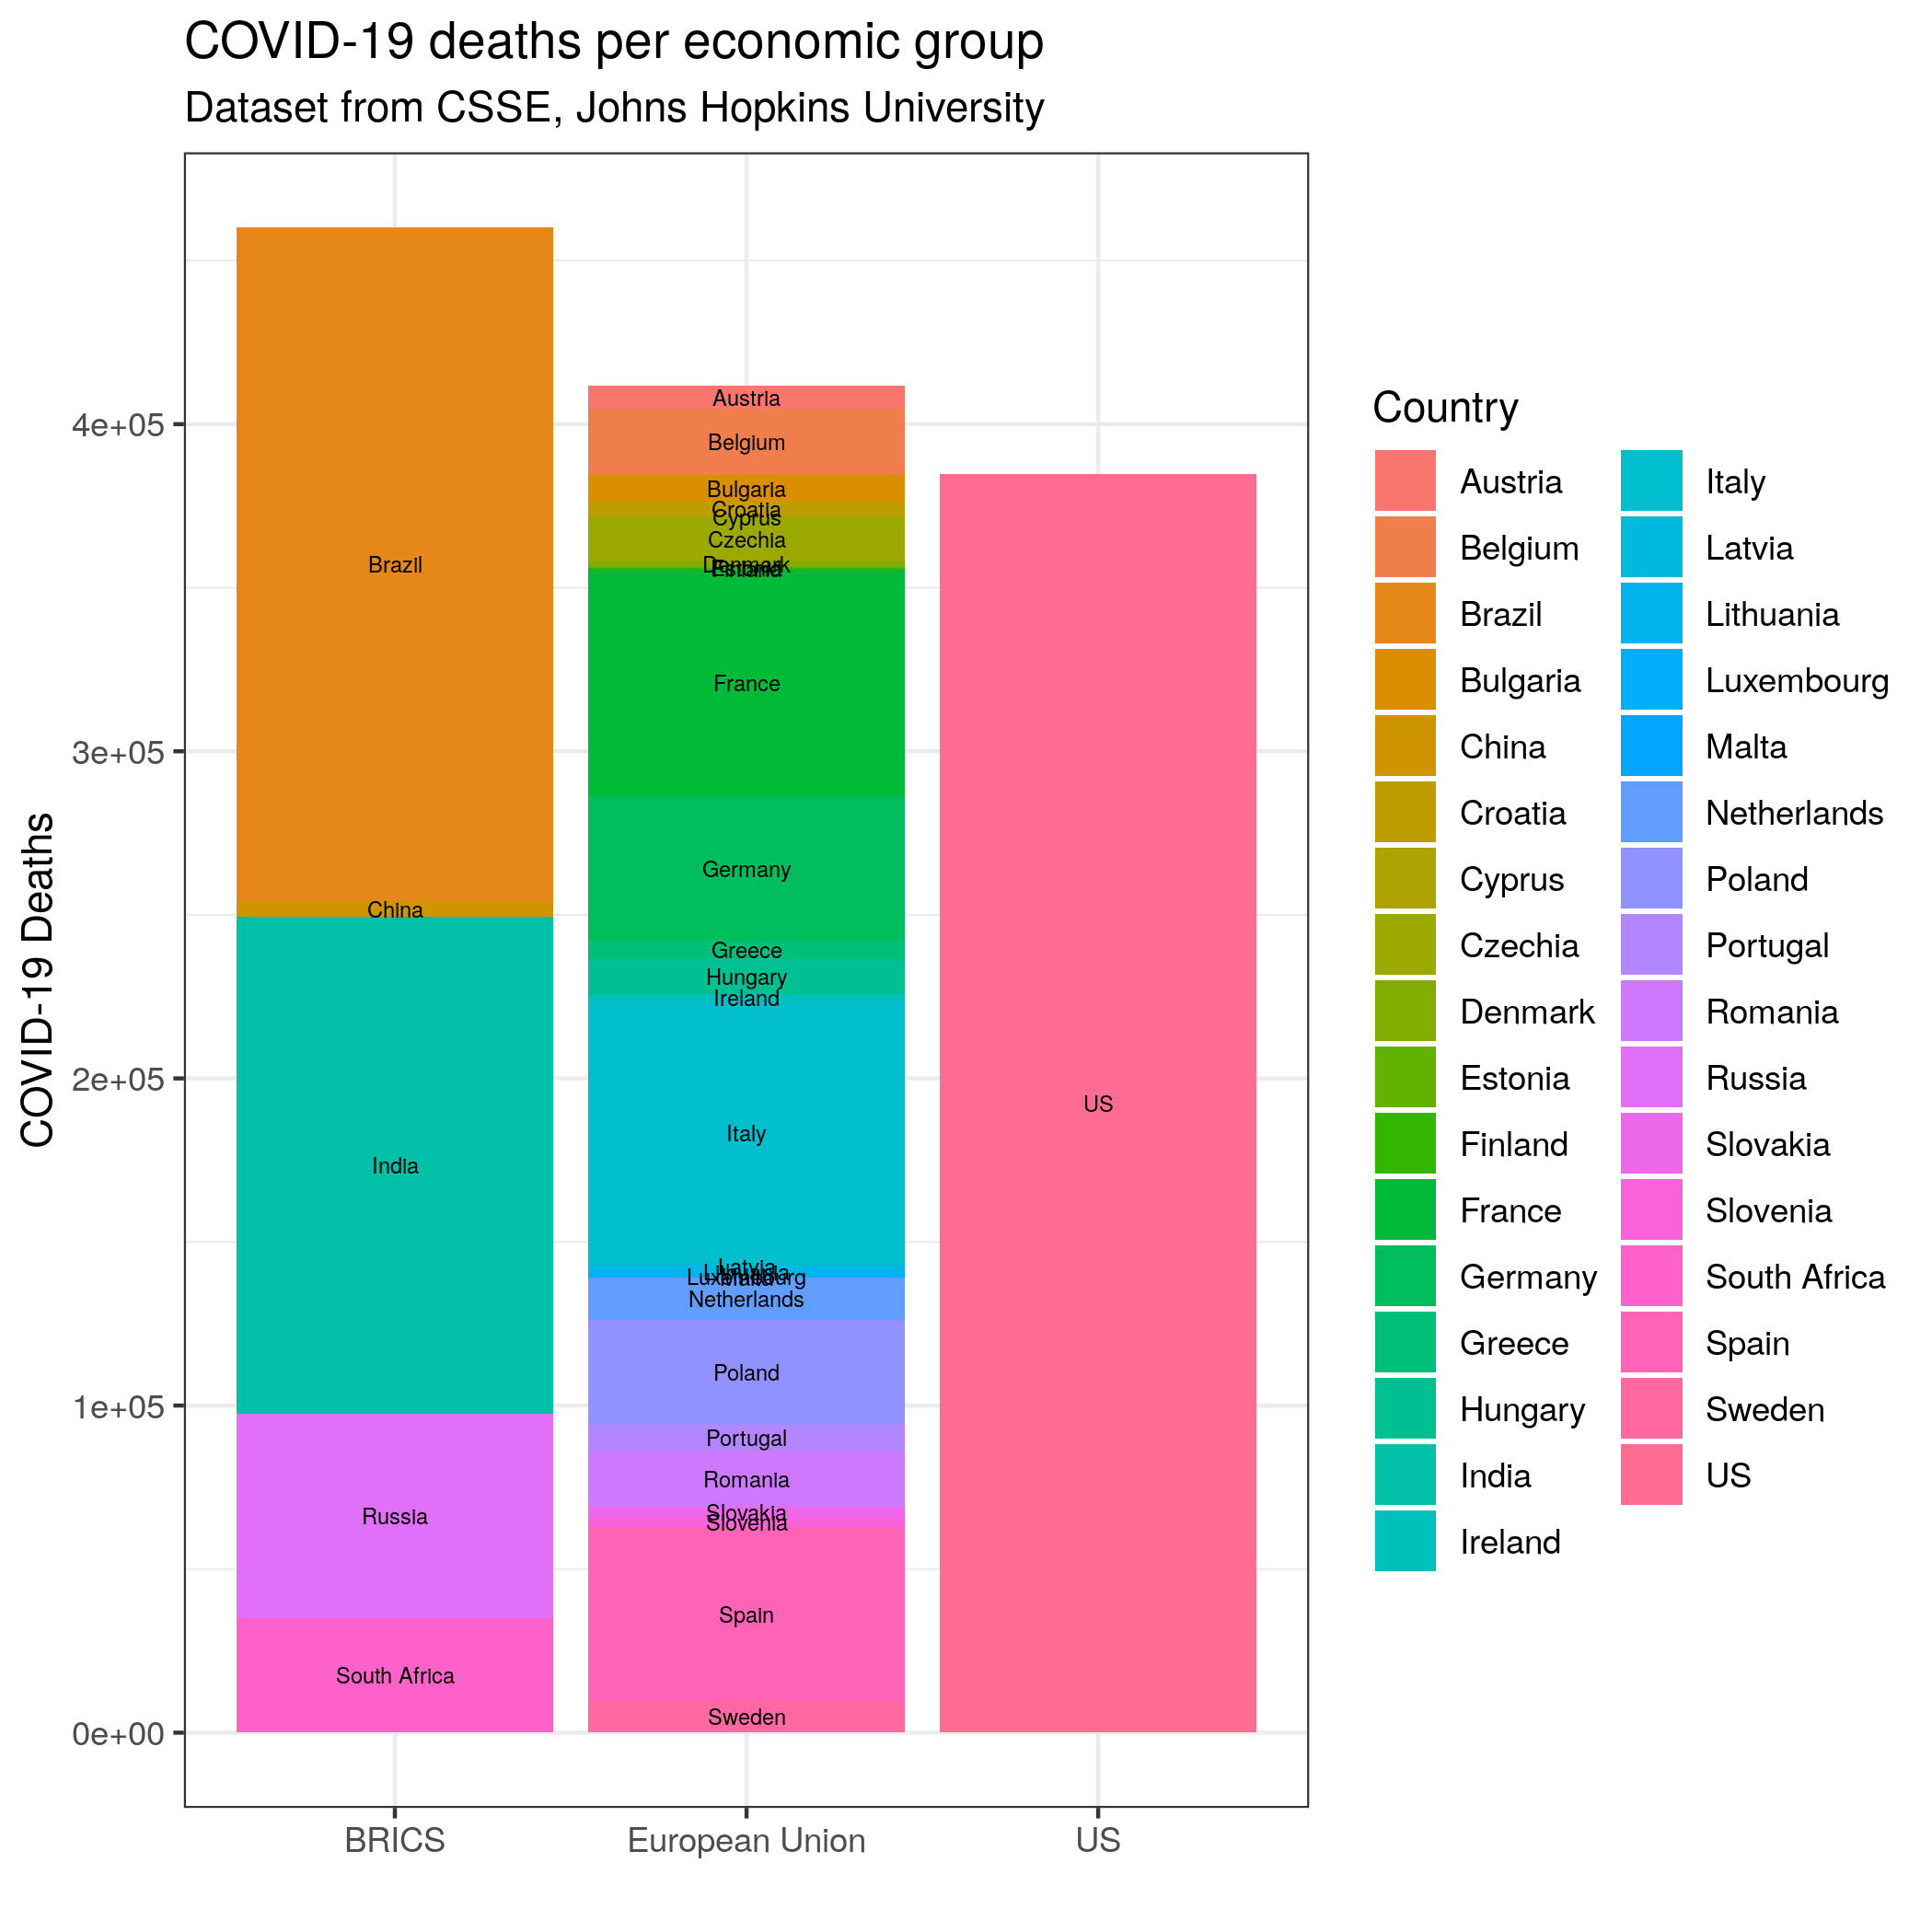
\includegraphics[width=1\linewidth]{images/aggr_econ_deaths.png}
  \captionof{figure}{COVID-19 deaths per economic group}
  \label{fig:aggr_econ_deaths}
\end{minipage}
\end{figure}

Finally, lines \ref{ratio_A}-\ref{ratio_Z} sort all countries (minus the reported cruise ships in the dataset) by their ratio of total COVID-19 confirmed cases to the total number of deaths attributed to the virus, and keep the worst $25$ of them.
These are merged with the joint stats of all previous groups of countries (both economic and geographic) and presented in Figure \ref{fig:aggr_lollipop}, each annotated with their actual number of deaths and confirmed COVID-19 cases.

\begin{figure}[H]
\centering
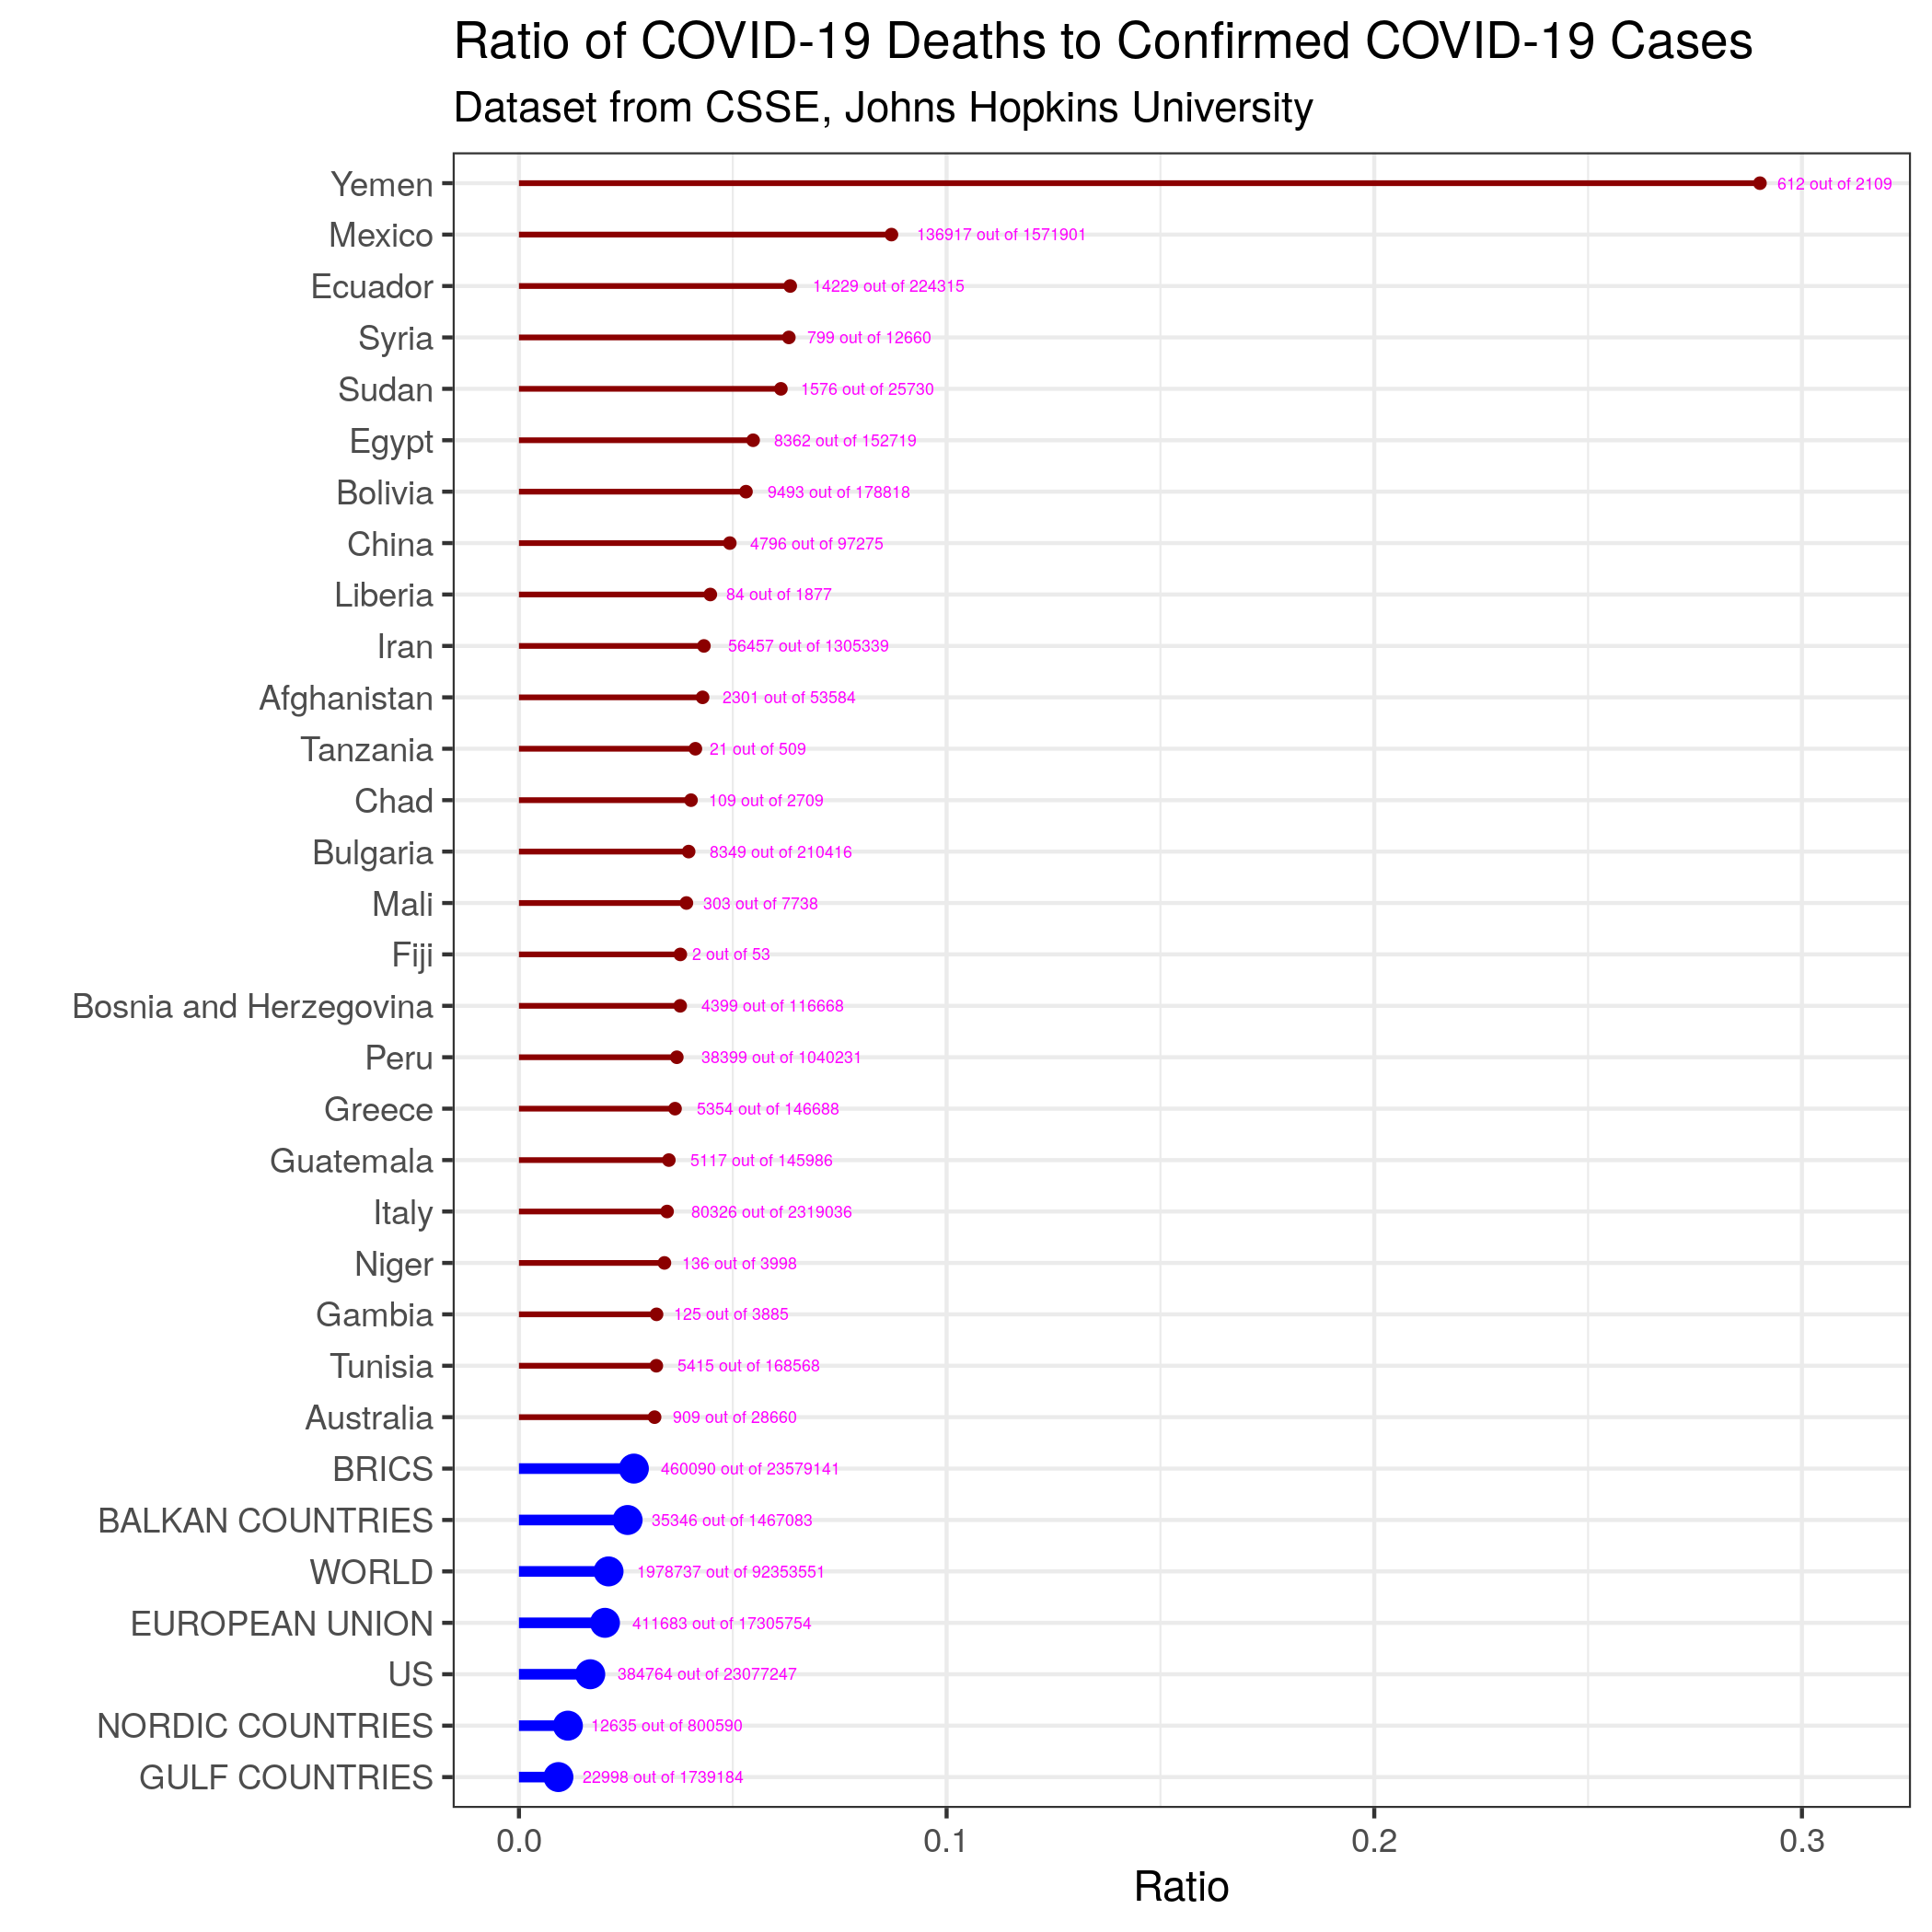
\includegraphics[width=1\linewidth]{images/aggr_ratio_lollipop.png}
\captionof{figure}{Ratio of COVID-19 Deaths to Confirmed COVID-19 Cases.}
\label{fig:aggr_lollipop}
\end{figure}

As it is made obvious by the diagram, countries that are either poor or isolated tend to have a higher ratio of deaths attributed to COVID-19 to confirmed cases of the virus, albeit larger countries, like Australia and Italy also appear in the bottom $25$ of them.
Sadly, Greece also appears in this list -- as a matter of fact it appears to be the third worst European country and the second worst within the European Union (after Bulgaria).

	\section{Seasons}

A quite common question related to COVID-19 is whether the seasons might affect the number of confirmed cases and the number of deaths all around the globe.
%One of the COVID-19 related questions I have always had is how the season might have affected the number of the confirmed cases and the number of the deaths all around the globe.
The dataset that we have in our disposal could actually allow me to answer this question, as long as we are capable of actually determining the season for each of the countries observed.


\subsection{Determining the Hemispheres}

To roughly determine the season of each country, we take advantage of one of the variables that we had earlier removed from our dataset, the Latitude, which should be enough to compare the velocity of the spread of the virus across countries with different seasons at a given time.
The function \texttt{determine\_hemispheres()}, which is shown below, given a \texttt{data.table} as returned by the \texttt{processing()} function that was explained earlier, returns it enriched with a new variable: \texttt{Hemisphere}.
Each observation can have three values for the \texttt{Hemisphere} variable: \texttt{Northern}, \texttt{Southern} or \texttt{Equator}, indicating whether an observation refers to a country located in the northern or southern hemisphere, or ±$10$ degrees from Earth's equator, respectively.

Note that in this case, where we know that our dataset is very small, we have developed a standalone function that performs the retrieval and processing of the \texttt{data.table} from scratch.
Had the dataset been bigger or our computing (or networking) capabilities restricted, we would probably refrain from doing so.
Instead, we would modify the initial data processing procedure to include this calculation as well.

%\begin{lstlisting}[language=R]
\begin{minted}[linenos=true, escapeinside=@@]{R}
determine_hemispheres <- function(dt) {
  lats <- fread(DEATHS_URL, header = TRUE,                    @\label{mntd01_dl1}@
                select = c("Country/Region", "Lat")           @\label{mntd01_dl2}@
    )[Lat != 0                                                @\label{mntd01_flt}@
     ][, .(lat = mean(Lat)), by = c("Country/Region")         @\label{mntd01_cntrymn}@
      ][, Hemisphere := as.factor(ifelse(lat > 10,            @\label{mntd01_cls_A}@
                                         "Northern",
                                         ifelse(lat < -10,
                                                "Southern",
                                                "Equator")))  @\label{mntd01_cls_Z}@
       ][, lat := NULL]                                       @\label{mntd01_cln}@
  setnames(lats, "Country/Region", "Country")                 @\label{mntd01_ren}@

  merge(dt, lats, by = c("Country"))                          @\label{mntd01_mrg}@
}
\end{minted}
%\end{lstlisting}

In the beginning (lines \ref{mntd01_dl1}-\ref{mntd01_dl2}), \texttt{determine\_hemispheres()} retrieves the columns of interest from one of the two CSV files of the dataset (the smaller between them, but this is not important) anew and filters out (line \ref{mntd01_flt}) any invalid observations (i.e., a couple of \texttt{N/A} and the two cruise ships included in the dataset).
It then calculates a ``mean" latitude for each country (by grouping by them (line \ref{mntd01_cntrymn}) -- recall that the original CSV includes multiple observations per country per date, according to the availability of data for each country's regions), and moves on to classify them based this value as \texttt{Northern}, \texttt{Southern} or \texttt{Equator} countries (lines \ref{mntd01_cls_A}-\ref{mntd01_cls_Z}).
Finally, it cleans the \texttt{data.table} from the temporary variable used for this classification (line \ref{mntd01_cln}), and merges the new \texttt{data.table} into the given one (line \ref{mntd01_mrg}), after properly renaming their common variable to \texttt{"Country"} (line \ref{mntd01_ren}).


\subsection{Visualization}

To visualize the data, a standalone function has been developed: \texttt{plot\_seasons()}.
Given a \texttt{data.table} as produced by \texttt{determine\_hemispheres}, after performing some additional calculations, it plots the time series data for the daily confirmed cases and the daily deaths per hemisphere, and stores the results to the local filesystem.
It is presented in the listing below and subsequently it is explained.

\begin{minted}[linenos=true, escapeinside=@@]{R}
plot_seasons <- function(dt) {
  hem_series <- dt[,                                         @\label{mntd02_sercr}@
                   .(confirmed.ind = sum(confirmed.ind),
                     deaths.inc    = sum(deaths.inc)),
                   by = .(date, Hemisphere)
                  ][,                                        @\label{mntd02_chain}@
                    ":="(confirmed = cumsum(confirmed.ind),
                         deaths    = cumsum(deaths.inc)),
                    by = .(Hemisphere)]                      @\label{mntd02_serend}@
  hem_sum <- hem_series[,                                    @\label{mntd02_hsum_A}@
                        .(confirmed = sum(confirmed.ind),
                          deaths    = sum(deaths.inc)),
                        by = .(Hemisphere)]                  @\label{mntd02_hsum_Z}@

  first_date <- hem_series[date == min(date), date][1]
  last_date <- hem_series[date == max(date), date][1]
  ggplot(data = hem_series) +                                @\label{mntd02_plt1_A}@
    aes(x = date, y = confirmed.ind, color = Hemisphere) +
    geom_line(size = .5) +
    geom_smooth() +
    aes(xmin = first_date, xmax = last_date) +
    scale_x_date(date_labels = "%b %Y",
                 limit = c(as.Date("2020-01-21"),as.Date("2021-01-19")),
                 expand = c(0, 0)) +
    scale_y_log10() +
    labs(title = "Daily confirmed COVID-19 cases") +
    labs(subtitle = "Dataset from CSSE, Johns Hopkins University") +
    labs(x = "", y = "") +
    theme_bw() +
  ggsave("hem_series_daily_cases.png")                       @\label{mntd02_plt1_Z}@
  ggplot(data = hem_series) +                                @\label{mntd02_plt2_A}@
    aes(x = date, y = deaths.inc, color = Hemisphere) +
    geom_line(size = .5) +
    geom_smooth() +
    aes(xmin = first_date, xmax = last_date) +
    scale_x_date(date_labels = "%b %Y",
                 limit = c(as.Date("2020-01-21"),as.Date("2021-01-19")),
                 expand = c(0, 0)) +
    labs(title = "Daily deaths due to COVID-19") +
    labs(subtitle = "Dataset from CSSE, Johns Hopkins University") +
    labs(x = "", y = "") +
    theme_bw() +
  ggsave("hem_series_daily_deaths.png")                      @\label{mntd02_plt2_Z}@
\end{minted}

The function starts with the creation of a \texttt{data.table} and a few calculations on it (via chaining).
A new \texttt{data.table} is created (\texttt{hem\_series}) (lines \ref{mntd02_sercr}-\ref{mntd02_chain}), which contains the daily confirmed cases and the daily number of deaths per \texttt{Hemisphere}.
Chained is the calculation of the respective cumulative variables (lines \ref{mntd02_chain}-\ref{mntd02_serend}), i.e., the cumulative number of confirmed COVID-19 cases as well as the cumulative number of deaths because of the virus.
Last, \texttt{hem\_sum} (lines \ref{mntd02_hsum_A}-\ref{mntd02_hsum_Z}) stores aggregate statistics calculated for each Hemisphere.
The respective plots for the cumulative variables and the aggregate statistics are not presented here, to adhere to the assignment's strict requirement to be at most $15$ pages long.

Subsequently, using \texttt{ggplot2} again (lines \ref{mntd02_plt1_A}-\ref{mntd02_plt1_Z} and \ref{mntd02_plt2_A}-\ref{mntd02_plt2_Z}), we plot the daily stats.
The results are presented in Figures \ref{fig:daily_cases_time} and \ref{fig:daily_deaths_time}.

\begin{figure}[H]
\centering
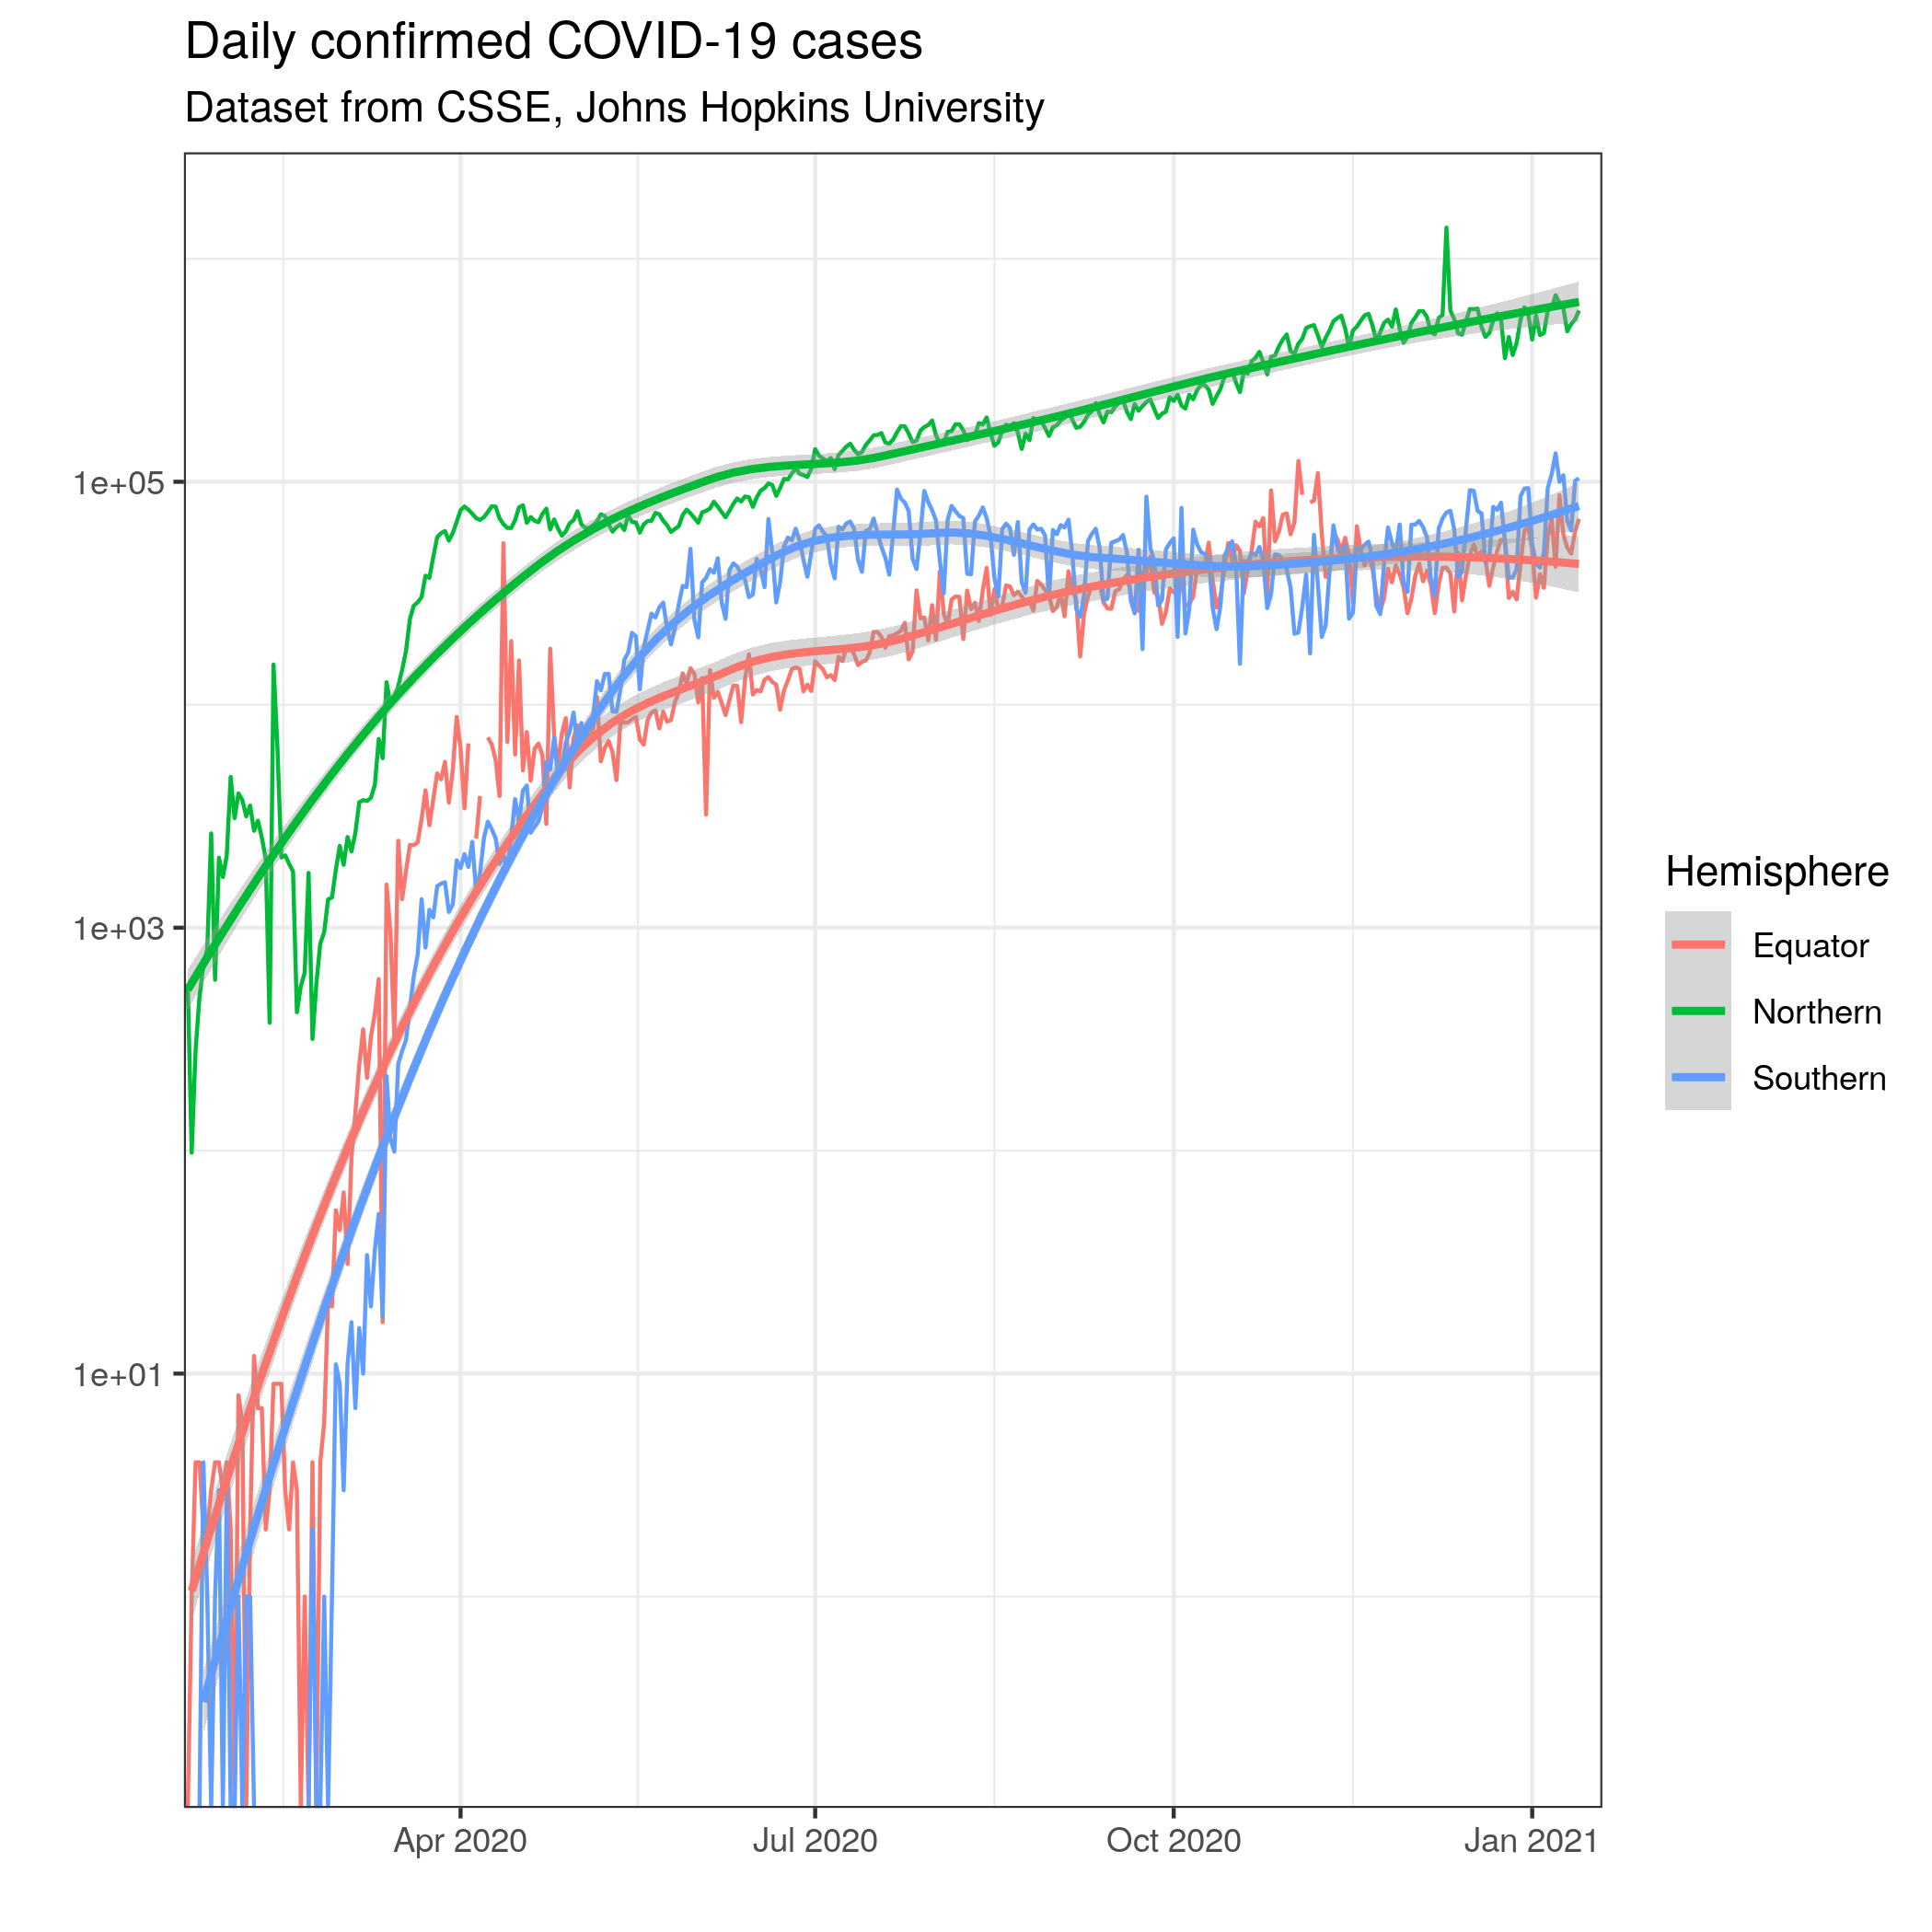
\includegraphics[scale=0.7]{images/hem_series_daily_cases.png}
\caption{Daily confirmed COVID-19 cases per hemisphere by season (in logarithmic scale).}
\label{fig:daily_cases_time}
\end{figure}

\begin{figure}[H]
\centering
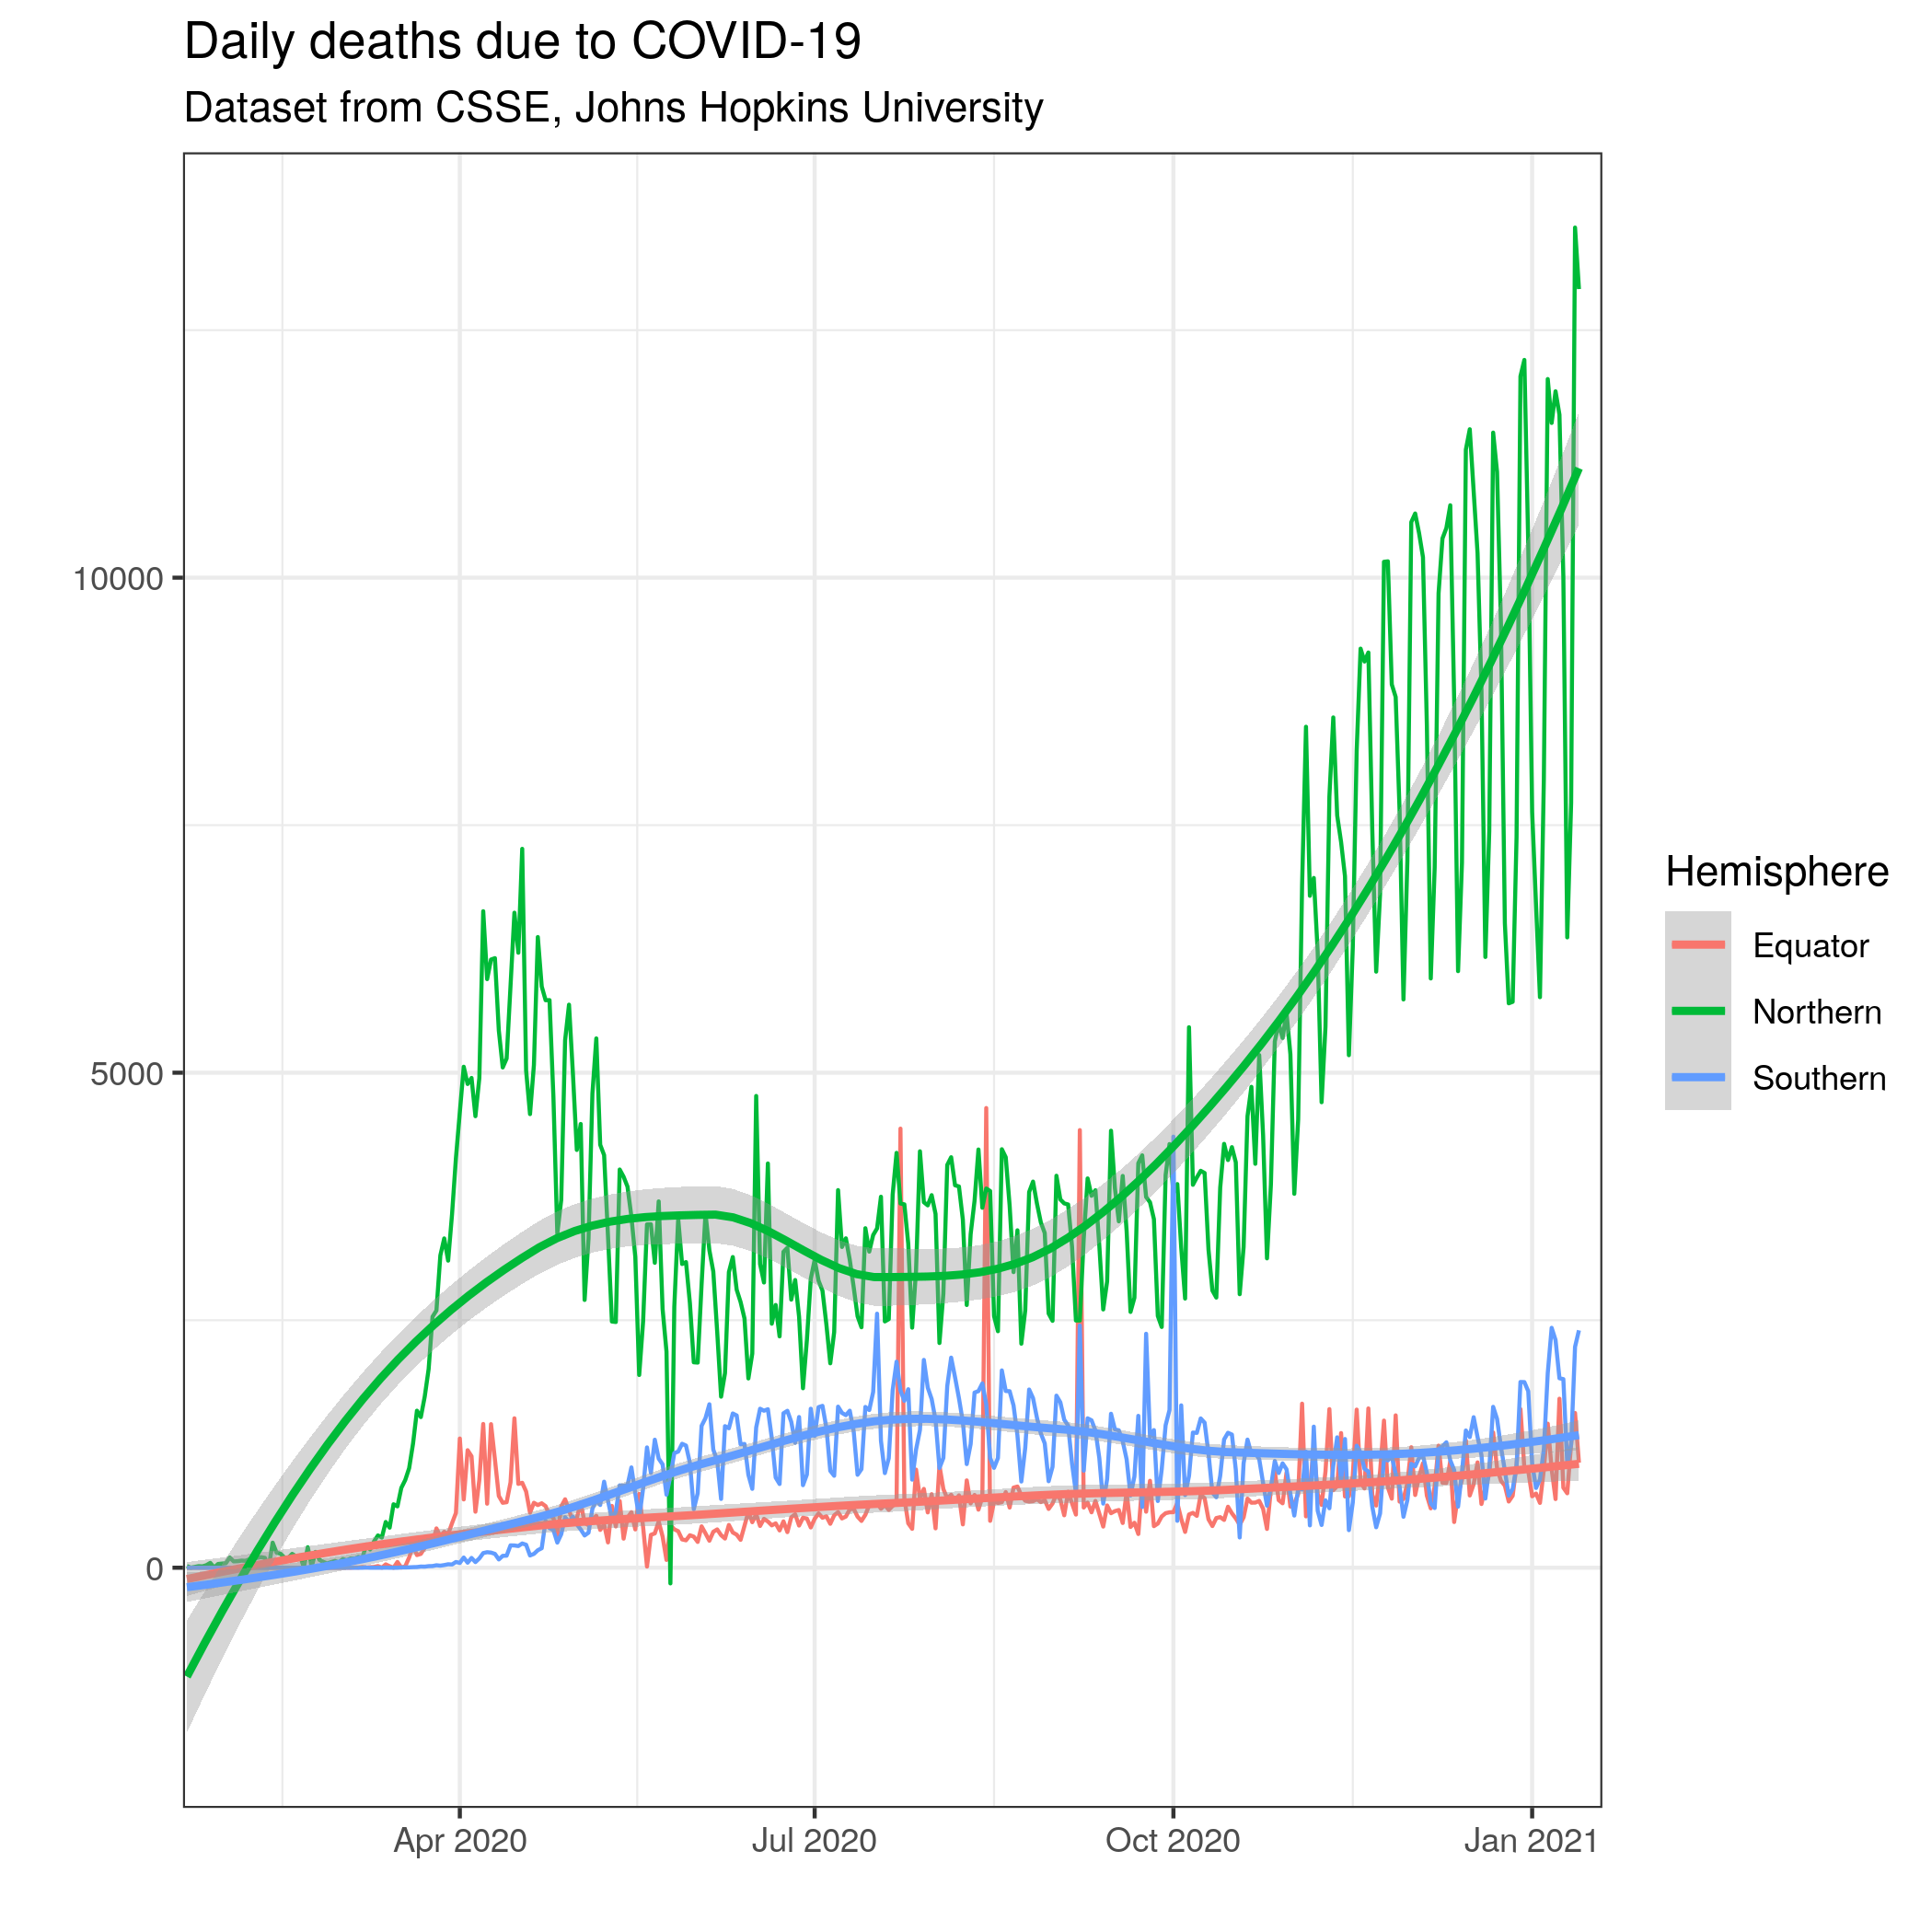
\includegraphics[scale=0.9]{images/hem_series_daily_deaths.png}
\caption{Daily COVID-19 deaths per hemisphere by season (in linear scale).}
\label{fig:daily_deaths_time}
\end{figure}


\subsection{Discoveries}

Judging from the figures above, we can verify our hypothesis that seasons affect the spread of the virus, but only up to a certain point.

As we can see in both diagrams, on June, July and August, both the confirmed COVID-19 cases and the daily number of deaths are increased for the southern hemisphere and either increased or at least stabilized for the northern hemisphere.
During these months countries of the southern hemisphere go through winter, whereas countries of the northern hemisphere go through spring.
On the other hand, later within the year things are getting worse for the countries of the northern hemisphere (as the winter approaches), while they seem to get better for countries of the southern hemisphere (where summer is getting closer and closer).

Countries on the equator appear to be only moderately affected by seasons in comparison with the other two groups.
Their plots indicates that they follow the general trend of the global spread of the virus more strictly than the other two groups.


\subsubsection{A Note on the Recent Spike}

At this point, it is worthwhile to comment on the obvious spike observed at the plot of confirmed cases for the northern hemisphere, which, had the plot been in linear scale, would definitely dominate the reader's attention with respect to the figure.
Judging solely by the figure, our first intuition was that it concerns some major social event that might have occurred a few days earlier and vastly increased the spread of the virus for a few days.
For instance, United States' Thanksgiving day could be one such social event, which takes place in late November.

Leveraging the power of R, we moved on to verify the hypothesis.
What follows is a sequence of R commands run in interactive mode that indicate the rationale of our attempts to find out a reasonable explanation for this spike.
If run in this order, their results back the conclusions that immediately follow them.

\begin{minted}{R}
> source("covid19-eda.R")
> tmp <- determine_hemispheres(processing()$dt)
> # Locate the incident:
> tmp[Hemisphere == 'Northern'][confirmed.ind == max(confirmed.ind)]
> # Explore the days before and after the incident:
> tmp[Hemisphere == 'Northern'][date == '2020-12-10'][order(-confirmed.ind)]
> tmp[Hemisphere == 'Northern'][date > '2020-12-1'][
+     date < '2020-12-20'][order(-confirmed.ind)][1:20]
> tmp[Country == 'Turkey'][date > '2020-12-1'][date < '2020-12-20']
> tmp[Hemisphere == 'Northern'][order(-confirmed.ind)][1:20]
\end{minted}

Even though for 18 out of the 20 days checked the US was indeed topping the daily confirmed cases stats (possibly explained by the preceding Thanksgiving), it turns out that the huge spike was caused by Turkey (with India being the country filling the last spot of the top 20 of this period).

After verifying the correctness of our own calculations, and to actively support the openness of data which enables information flows and improves the knowledge overall, our first thought was to contact the team catering the dataset to address the issue.
%To our great surprise (and our even greater relief), it turns out that this issue is well-known, and as a matter of fact exists as a standalone announcement in the form of a dedicated GitHub Issue\cite{ghcsse3484} at the repository at hand.
To our great surprise (and relief), it turns out that this issue is well-known, and as a matter of fact exists as a standalone announcement in the form of a dedicated GitHub Issue\cite{ghcsse3484} at the repository at hand.
In brief, during that period Turkey had recently changed the criteria for qualifying a patient as a COVID-19 case.
%To rectify their thus far statistics, Turkey reported \textit{all} of its past historical data in addition with the actual data within a single day ($823225$ confirmed cases on December 10th, 2020), thus causing the huge observable spike across the whole Hemisphere's data.
To rectify their statistics thus far, Turkey reported \textit{all} of its past confirmed cases (according to the new criteria) as new data within a single day ($823225$ confirmed cases on December 10th, 2020 alone), hence causing the big spike across the whole Hemisphere's data.


    \pagestyle{empty}
    %\newpage  %% (Un)comment to toggle `Bibliography` being on a separate new page
    \nocite{*}
    \bibliographystyle{ieeetr}
    \renewcommand{\refname}{References}
    \bibliography{references}
\end{document}
